%%%%%%%%%%%%%%%%%%%%%% file bookchapter.tex %%%%%%%%%%%%%%%%%%%%%%%%%
%
%%%%%%%%%%%%%%%%%%%%%%%%%%%%%%%%%%%%%%%%%%%%%%%%%%%%%%%%%%%%%%%%%%%
\documentclass[runningheads,a4paper]{llncs}

\usepackage{amssymb}
\usepackage[intlimits]{amsmath}
\setcounter{tocdepth}{3}


%\usepackage{cmap}
\usepackage[T1]{fontenc}
%\usepackage{graphicx}
\usepackage[english]{babel}
\usepackage{cite}
%\usepackage{subfig}
\usepackage{adjustbox}
\usepackage{tikz}
\usepackage{siunitx}
%\usepackage{subcaption}
\usepackage{caption}
\usepackage{chemfig}
%\usepackage{subfigure}
%\renewcommand{\thesubfigure}{(\Alph{subfigure})}
\usetikzlibrary{calc,arrows,shapes,shapes.geometric,decorations.pathmorphing,patterns}
\usepackage{moreverb}
\usepackage{acronym}
\usepackage{float}

\usepackage{lscape}
\usepackage{geometry}
\usepackage{pdflscape}

\usepackage{url}
\newcommand{\code}[1]{\texttt{#1}}
\newcommand{\keywords}[1]{\par\addvspace\baselineskip
\noindent\keywordname\enspace\ignorespaces#1}


\makeatletter
%\renewcommand{\fnum@}{Figure \thefigure}
\makeatother

\begin{document}

\mainmatter  % start of an individual contribution

% first the title is needed
\title{Building Towards the Future in Chemical and Materials Simulation with Accessible and Intelligently Designed Web Applications}

% a short form should be given in case it is too long for the running head
\titlerunning{EMSL Arrows and TinyArrows}

% the name(s) of the author(s) follow(s) next
%
%\author{Eric J. Bylaska, Duo Song}
%}
%
% (feature abused for this document to repeat the title also on left hand pages)

% the affiliations are given next; don't give your e-mail address
% unless you accept that it will be published
%\institute{Physical Sciences Division, Pacific Northwest National Laboratory, Richland, WA 99354}
\author{Eric J. Bylaska\inst{1}\orcidID{0000-0001-6405-599X} \and
Duo Song\inst{1} \and 
Eugene S. Ilton\inst{1} \and
Shaun O'Leary\inst{2} \and
Tifany L. Torralba-Sánchez\inst{3} \and
Paul G. Tratnyek\inst{3}
}
%
\authorrunning{E.J. Bylaska et al.}
% First names are abbreviated in the running head.
% If there are more than two authors, 'et al.' is used.
%
\institute{
Physical Sciences Division, Pacific Northwest National Laboratory \\
Richland, WA 99354, USA \and
Research Computing Division, Pacific Northwest National Laboratory \\
Richland, WA 99354, USA \and
OHSU-PSU School of Public Health (Mailcode HRC-3), Oregon Health & Science University (OHSU), 3181 SW Sam Jackson Park Road \\
Portland, Oregon 97239-3098, USA\\
\url{https://arrows.emsl.pnnl.gov/api}\\
\url{https://github.com/ebylaska/TinyArrows}
}


\maketitle

%%%% Not sure if abstract is needed?? %%%%
\begin{abstract}
 Over the last few decades, significant progress has been made in the development and use of electronic structure and other molecular simulation methods.  As these methods become more mature and are able to simulate larger and more complex chemical simulations, the need for improvement in scientific visualization, molecular builders, simplified input to simulation methods,  and the development of new approaches and languages to describe simulations, along with workflows to carry them out, becomes more apparent.  
 In this chapter, we describe our recent efforts in developing a prototype open-source computational tool called Arrows that combines NWChem, SQL and NoSQL databases, email, web APIs, and web applications in a way that makes molecular and materials modeling accessible to all scientists and engineers.  At the same time, because of its simplified input, it provides a framework for expert users to carry out large numbers of calculations and run complex workflows.
\end{abstract}

\begin{keywords}
Computational chemistry workflows, molecular builders, JSMol, NWChem, Mopac, DFT, CCSD(T), Plane-Wave DFT, PAW, PSPW, Chemistry, Ab initio Molecular Dynamics, AIMD, AIMD/MM, QM/MM, AIMD-EXAFS, hematite, Zn(II), carbon tetrachloride, trichloropropane, 2,4-dinitroanisole, DNAN, hydrolysis, hydrogenolysis, reaction pathways, kinetics, reaction prediction
\end{keywords}

\section{Introduction}
\label{sec:Introduction}
Computational chemistry has played a large and growing role in chemistry, material science, and biology, since the appearance of the first electronic computing systems and subsequent programmable computers in the early to mid-part of the last century.  Some of the first calculations, which were used to generate atomic form factors for X-ray and electron scattering~\cite{cromer1965scattering}, had an immediate scientific impact that continues to this day.  From these beginnings, the growth and impact of the field has continued, %steadily, 
so much so, that today it has become a necessary tool across multiple domains of science and engineering.  This is an extraordinary impact for a field still undergoing rapid development. In fact, recent economic analysis concluded that molecular modelling contributes $\sim 1\%$ of the GDP of a large technologically advanced country~\cite{goldbeck2012economic}.  %This remarkable for a scientific field that is still in an embryonic state.
%and that relies on a handful of (mostly academic) computer programs in which the computational methods have reached a significant level of matand that relies on a handful of (mostly academic) computer programs in which the computational methods have reached a significant level of mat


%\begin{figure*}[!h]
%   \centering
%   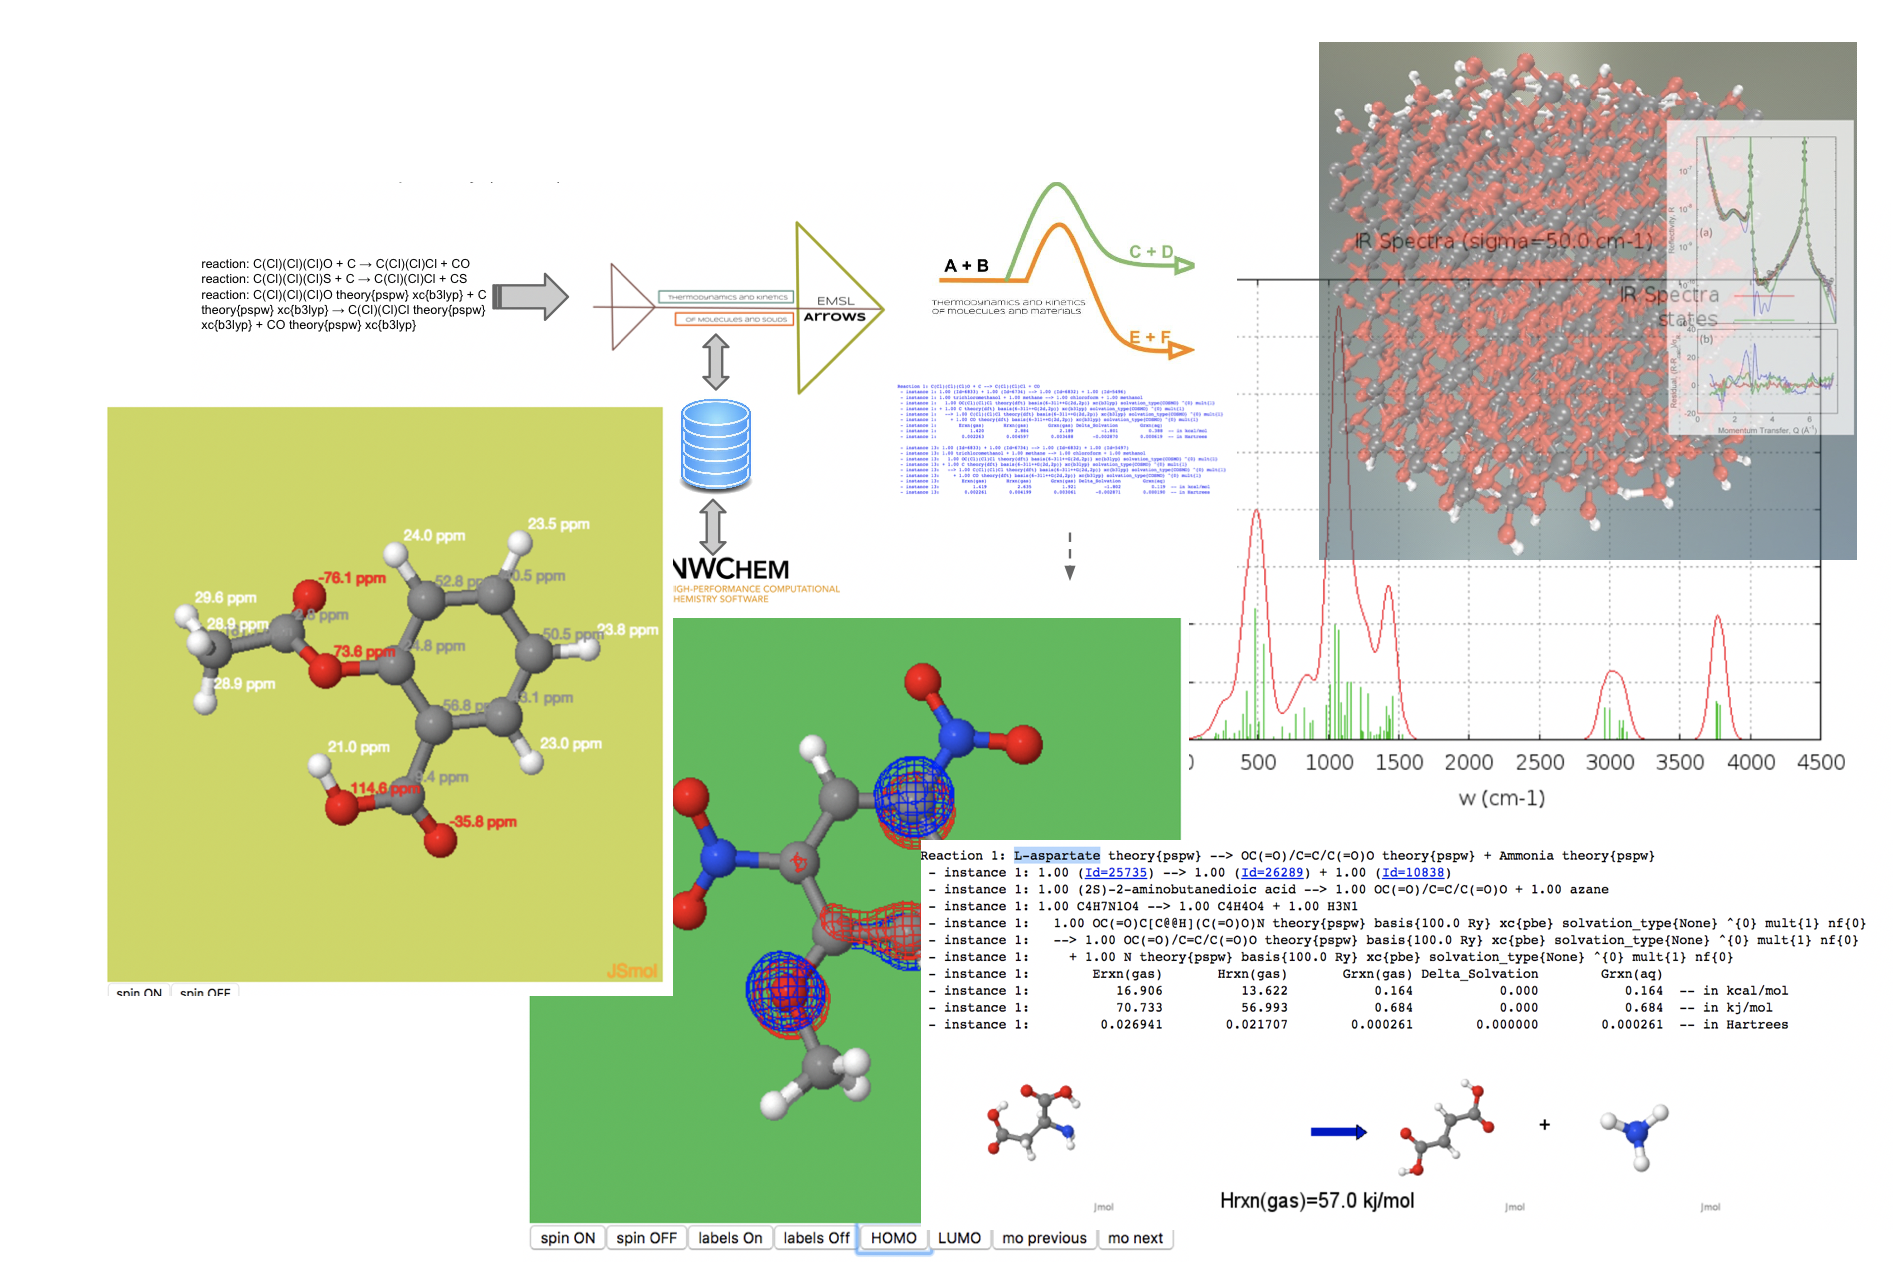
\includegraphics[width=\textwidth]{images/arrows.png}
%   \caption{Illustration of the capabilities of the Arrows web tool.}
%   \label{fig.intro.arrows}
%\end{figure*}

The success and versatility of computational chemistry is partly due to increases in processing power coupled with advances in algorithms and software.  With these advances, computational chemistry is now able to probe various physical observables through the use of predictive atomic level simulations.  
Combined with the freedom to utilize diverse external constraints and fields, these methods are able to explore larger spatial and time scales of chemical processes under a variety of conditions. Given this versatility, along with the new insight
that comes from having an atomic picture of processes, not easily obtained from experiment, it is already very common to augment experimental studies with simulation.  For example, simulation is actively used in the interpretation of molecular spectroscopies.  It is also actively used to systematically and efficiently extend experimentally measured thermodynamic and kinetic properties of chemical systems.
However, augmenting and replacing experiment with simulation is nontrivial, since simulating new materials is complicated by the sensitivity of the processes at the macroscopic scale to the atomic scale; the unusual and unexpected bonding behaviors of materials; cases where extreme temperature and pressure environments could be encountered; and the requirements that simulations be as parameter free as possible and extremely reliable. 

The tools of electronic structure theory and statistical mechanics combined with advanced parallel packages such as NWChem~\cite{kendall2000high,valiev2010nwchem,apra2020nwchem,kowalski2021nwchem} have proved to be very effective and productive computational chemistry methods. Indeed, computer programs that implement these types of methods consume a large fraction of supercomputer cycles.  Even with these hugely successful developments, reliable calculations of this type require considerable theoretical expertise, computational effort, and often costly software licenses that are out of reach for many scientists, engineers, and students. 

One of the biggest barriers to using computational chemistry is the need for efficient and intuitive input to the software.   This is particularly true for open-source programs such as NWChem that are trying to stay on the cutting edge with the latest theoretical and computational developments, and as a result the complexity of these programs continues to grow unabated. For example, NWChem implements a robust and diverse set of molecular theories, including Gaussian basis set DFT, high-level chemistry methods (e.g. MP2~\cite{moller1934note}, CCSD(T)~\cite{bartlett1994applications,bartlett2007coupled}), molecular dynamics (MD)~\cite{allen2017computer}, hybrid quantum mechanics/molecular mechanics (QM/MM), plane-wave density functional theory (DFT)~\cite{bylaska2017plane}, ab initio molecular dynamics (AIMD), and hybrid ab initio molecular dynamics/molecular dynamics (AIMD/MM)~\cite{laio2002hamiltonian,cauet2010structure} that can estimate the thermodynamics, kinetics, and spectra for molecules, nanoparticles, bio-materials, and minerals.  It arguably has the most capabilities of any molecular modeling code today.  As a result, new users of NWChem and other computational chemistry programs may feel like they need to take classes on how to use them, or at the very least obtain a certification akin to what used to be thought of as compulsory to use VisiCalc and Lotus spreadsheets in the 1980's.  

In addition to the input challenge, other problems with NWChem and other computational chemistry codes are that:
\begin{itemize}
\item Molecular modeling software is extremely complex, contains millions of lines of code, takes a long time to set up and to learn how to use. 
\item Even the most basic input for molecular modeling software requires the use of other software to generate it.
\item It is not uncommon for simulations to take days, weeks and even months to complete.
\item Multiple simulations are usually needed to calculate molecular properties and reaction energies. 
\item Because of this complexity, people unnaturally identify with codes and molecular theories, and they are hesitant to learn new codes and new molecular simulation techniques. 
%\item As a consequence, NWChem and other molecular modeling programs are not yet used by large numbers of scientists, engineers, and students who could benefit from using them.
\end{itemize}

\begin{figure*}[!h]
   \centering
   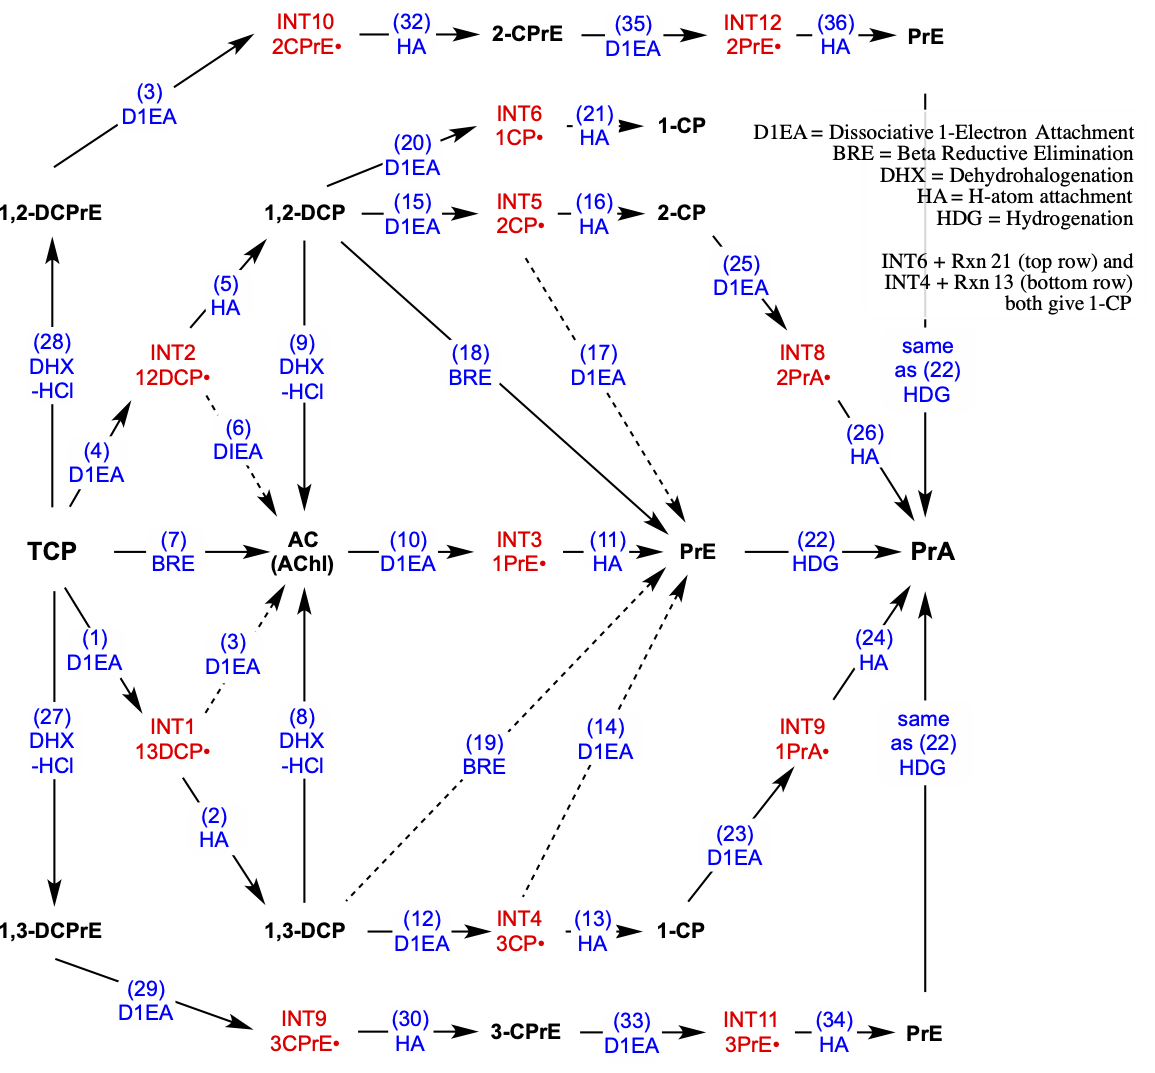
\includegraphics[width=1.0\textwidth]{images/tcp-sanchez.png}
   \caption{Example of a reaction network in environmental chemistry from work of authors.  Likely reactions for trichloropropane (TCP) under reducing conditions. Reaction network image in figure from Torralba et al.~\cite{torralba2020reduction}.}
   \label{fig.intro.rxnnetwork}
\end{figure*}
Many groups have been trying to fill this need by developing molecular graphics programs, graphical user interfaces (GUIs), and workflows~\cite{johnson1965ortep,wasikowski1993xmol,Unichem,michalewicz1995combining,baldridge1995qmview,smith1995molview,humphrey1996vmd,bode1998macmolplt,kokalj1999xcrysden,frisch2000gaussview,schaftenaar2000molden,portmann2000molekel,gans2001qmol,bahn2002object,schuchardt2002ecce,kokalj2003computer,gdanitz2005registering,verstraelen2008zeobuilder,thomas2010ccp1,hanson2010jmol,momma2011vesta,hanson2013jsmol,hanwell2021open,larsen2017atomic,nguyen2018nglview,smidstrup2019quantumatk,gilbert2019introduction,bienfait2013jsme,chen2012construction} and standardized formats to make molecular and materials data machine-readable and writable~\cite{murray2011cml,murray2011semantics,de2013data}. While extremely useful, these interface programs, which are hard to design and implement, sometimes end up being too narrowly focused and at the same time just as complicated to use as the underlying molecular modeling software.  Unfortunately, even with the plethora of available GUIs it is not uncommon for a user of quantum molecular modeling software (especially open source software) to become overwhelmed by the proemial state of the software, and having to resort to using multiple GUIs just to run a basic calculation. For example, to perform a simple DFT calculation for a molecule with an open source code like NWChem~\cite{kendall2000high,valiev2010nwchem,apra2020nwchem,kowalski2021nwchem}, one may have to use separate steps to build the molecule, fetch a basis set or pseudopotentials from a website, pre-optimize the molecule with a molecular force field or semi-empirical theory, submit and manage the DFT calculation, and lastly visualize the results.  

To make matters worse, when performing chemical studies, one rarely just needs the results of a single molecular calculation; in fact, it is very common to carry out many hundreds to thousands of molecular calculations.  As shown in Fig.~\ref{fig.intro.rxnnetwork}, this can be true even for chemical studies involving relatively simple molecules, like the degradation of chlorinated hydrocarbons in natural ground waters.

In response to these challenges, we have been investigating and prototyping intelligently-designed web interfaces to carry out complex and difficult chemical and materials simulations, while at the same time developing simplified input to make these simulations accessible to more scientists, engineers, and students.  In this chapter, an overview of the open-source computational chemistry and materials tool called Arrows is presented.  Arrows is a web tool that combines NWChem, SQL~\cite{chamberlin1974sequel,hursch1988sql} and NoSQL~\cite{stonebraker2010sql} databases, email, back-end web servers, external web services, and web applications to perform molecular and materials modeling from a web browser. There are two implementations of Arrows called EMSL Arrows and TinyArrows.  EMSL Arrows~\cite{emslArrows} is hosted by the William R. Wiley Environmental Molecular Sciences Laboratory (EMSL) at the Pacific Northwest National Laboratory (PNNL)~\cite{foster2005environmental,emslpnnl}, and TinyArrows is a stand-alone implementation of Arrows available on GitHub.


\section{Evolution of Chemical and Materials Computation}
\label{sec:Evolution}
Scientific computing is undergoing its biggest transition in over 60 years.  The old way in which scientific computations were performed was by modelers and technicians who had specialized access to large and mid-scale computers at scientific user facilities.  The new way will be for scientific calculations to be carried out by individual non-specialized scientists (and AI engines) using smart web 4.0~\cite{patel2013incremental} (web 5.0) interfaces, where the computing is carried out across a federated network of computers instead of at scientific user facilities. How we think about scientific computing is changing.  
\begin{itemize}
   \item  In the old way: 
   \begin{itemize}
      \item Computation was expensive. 
      \item Most computing cycles were obtained from scientific user facilities that were expensive to build and operate.
      \item In this hegemonic system based on scarcity, calculations were primarily carried out by experts, running difficult and large numbers of calculations.
      \item Routine simulations supporting single investigator scientific studies were given low priorities.
    \end{itemize}
   \item In the new way:
   \begin{itemize}
       \item Bezos’s Law~\cite{bezoslaw1,bezoslaw2,zia2017adaptive,weinman2014nuances,lin2015big} - The price of a unit of computing power decreases by approximately one-half every three years.
       \item Cloud computing and client-side computing  will be where we get many of our cycles.
       \item Most calculations will be automated and easy to carry out with the help of smart AI assistants.
       \item As computational resources become more available and upend 
       the system based on scarcity, modelers will be more than just be gatekeepers to computing cycles and providers of expert codes. They will be tasked with exploring scientific hypotheses through simulation.
       \item Modern web technologies will play a critical role in carrying out future scientific simulations. 
   \end{itemize}
\end{itemize}

These are big changes, but even bigger changes are to be expected with the rapid development and deployment of new web based technologies combined with database, artificial intelligence (AI), machine learning (ML), and other types of expert system software, making it possible to control devices, organize and plan work, and monitor events remotely.


A common term that encompasses most modern web technologies is "HTML5".  It refers to the fifth and latest version of HTML (Hyper Text Markup Language) for creating web pages that are more interoperable than in the past~\cite{htmlliving}.  Besides improving the markup available for web documents, it also introduces into the standard, various application programming interfaces (APIs), designed to work with low-powered devices, to help programmers build more robust and efficient web (and cross-platform mobile) applications.  New features include advanced vector graphics (notably a full implementation of OpenGL through WebGL~\cite{danchilla2012beginning,rego20153dmol}), audio (<audio> HTML element), video (<video> HTML element), and voice recognition (Web Speech~\cite{adorf2013web}).  There is even available software that implements a flexible database (indexedDB~\cite{collins2012indexed,kimak2015role}).  While HTML5 is still being developed and at the moment there is no browser that it fully supports, however, this situation has significantly improved in recent years, and many of its new features are now supported on most major web browsers.

Now that HTML5 is widely available, the time is right for computational chemistry to evolve from being a tool used only by specialists to a tool used by all chemists, material scientists and other scientific and engineering researchers.  A strength of molecular modeling, in particular electronic structure methods, that make it viable to  new ways of computing is the development of many human-readable and machine-readable input and output formats (e.g., geometry formats: SMILES~\cite{weininger1988smiles,weininger1989smiles}, IUPAC names~\cite{favre2013nomenclature}, common names, InChI~\cite{heller2009iupac,heller2013inchi,heller2015inchi}, InChIKey~\cite{heller2009iupac,southan2013inchi}, PDB~\cite{westbrook2003pdb}, XYZ, mol, ...; input and output formats: POSCAR~\cite{ong2013python}, CIF~\cite{hall1991crystallographic}, gau, gam, nw, ...;  number formats: CAS, KEGG numbers~\cite{kanehisa2000kegg}, CID~\cite{kim2016pubchem}, CSID~\cite{williams2014royal,ayers2012chemspider}, ChEMBL~\cite{gaulton2017chembl}, EC Number~\cite{bairoch2000enzyme}, DrugBank~\cite{wishart2006drugbank}, ICSD~\cite{hellenbrandt2004inorganic}, ...), and various standard acronyms to describe various calculation details such as theories (e.g., CCSD(T)~\cite{bartlett1994applications,bartlett2007coupled}, MP2~\cite{moller1934note}, DFT~\cite{hohenberg1964inhomogeneous,kohn1965self}, HF~\cite{roothaan1960self}, PSPW~\cite{bylaska2017plane}, MCSCF~\cite{schmidt1998construction}, and CI~\cite{szabo2012modern,ross1952calculations}), basis sets and exchange correlation functionals(e.g. 6-31G*~\cite{francl1982a,gordon1982a,hariharan1973a,hehre1972a}, 6-311++G(2d,dp)~\cite{clark1983a,francl1982a,krishnan1980a,mclean1980a,spitznagel1987a} B3LYP~\cite{beck1993density,lee1988development}, PBE0~\cite{adamo1999toward}, M06-2x~\cite{zhao2008m06}, LDA~\cite{vosko1980accurate}, PBE~\cite{perdew1996generalized}, and BLYP~\cite{becke1988density,lee1988development}), and simulation methods (e.g., AIMD, NEB~\cite{jonsson1998nudged}, DOS~\cite{ashcroft1976solid}, PDOS, BSSE~\cite{van1994state}, DIIS~\cite{pulay1980convergence}, and COSMO~\cite{klamt1993cosmo}).  This strength is also one of its weaknesses, as the downside to all these formats is it gives the appearance that input for molecular modeling is complicated and requires extensive expertise to use.

Input does not need to be complicated, and extensive software expertise should not be required for most molecular modeling calculations.  Every scientist and engineer has been trained to write balanced chemical reactions in their high-school chemistry class.  Indeed, it is possible to use optical chemical structure recognition (OCSR) to recognize handwritten chemical reactions, although these tools probably won't be completed and widely available for a few years~\cite{mcdaniel1992kekule,casey1993optical,rajan2020review,oldenhof2020chemgrapher}.  
%\begin{figure*}[!h]
%   \centering
%   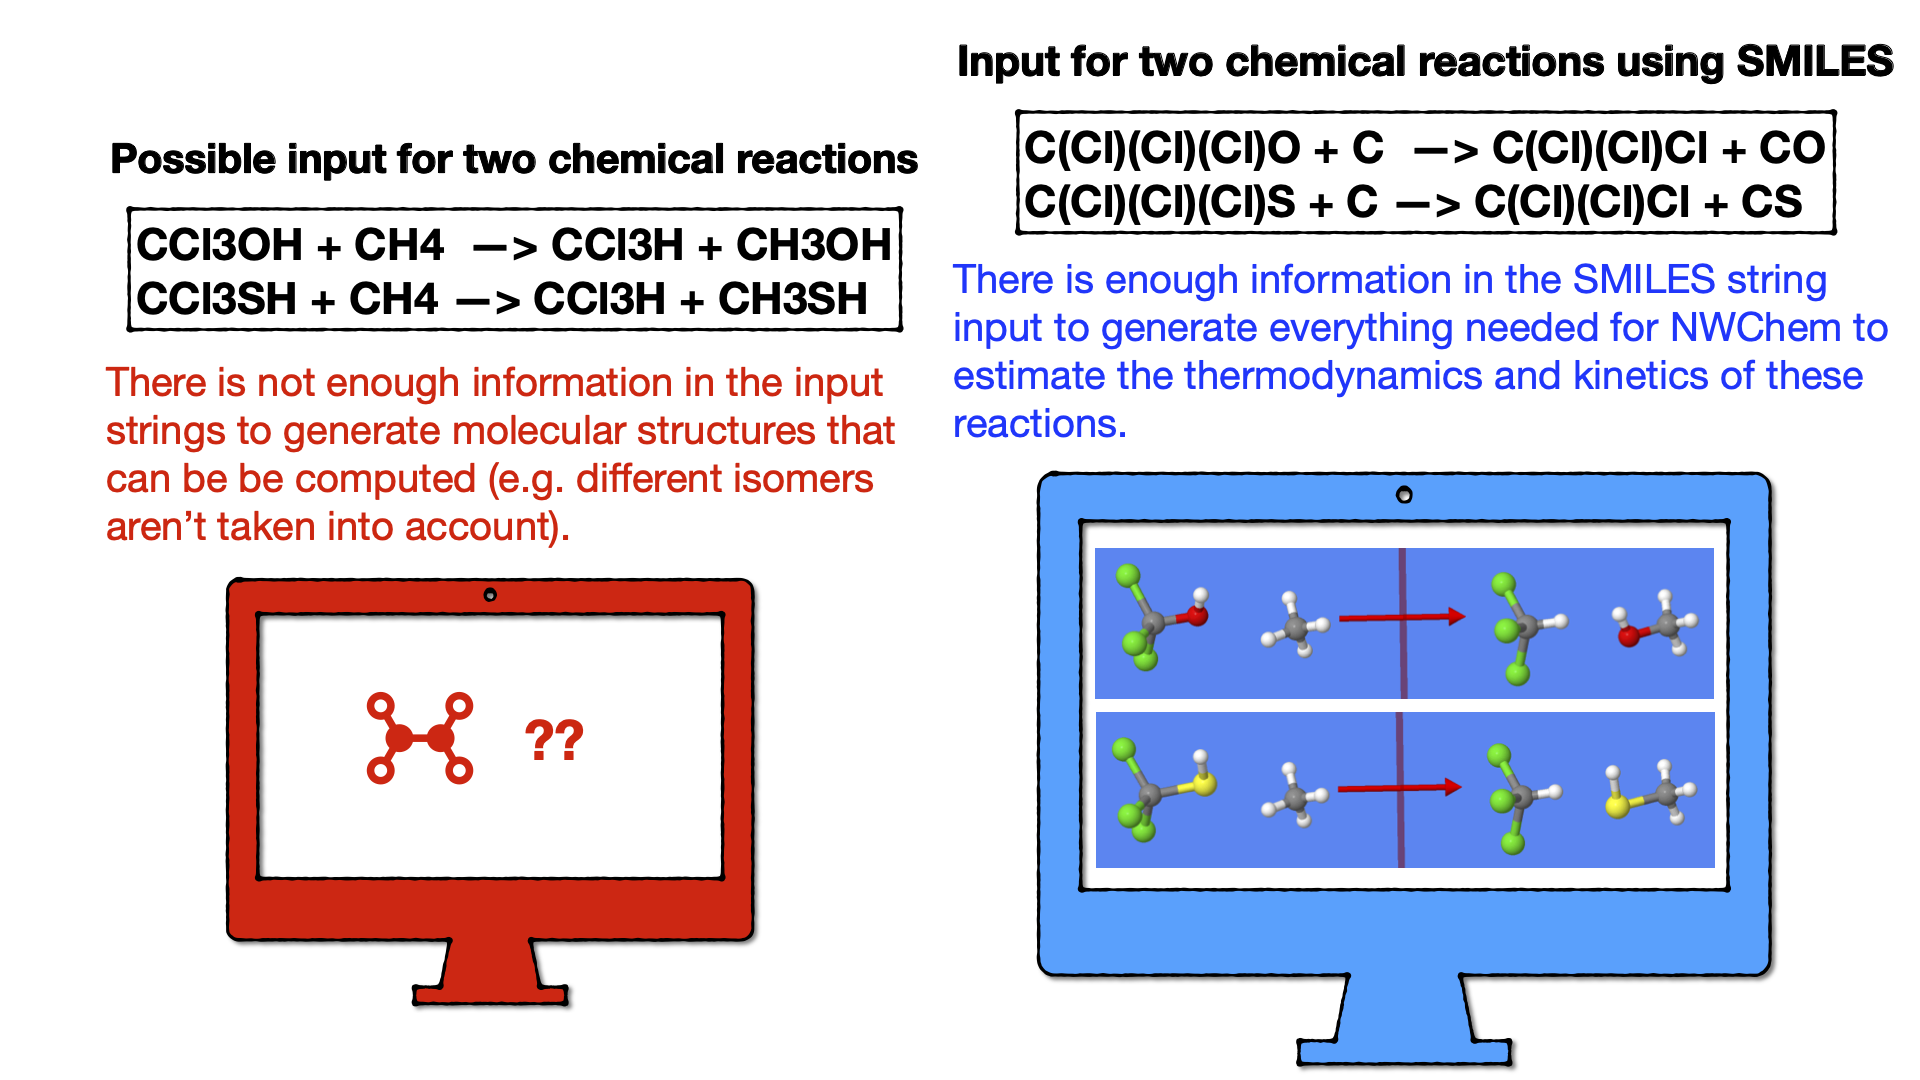
\includegraphics[width=\textwidth]{images/smilesinput4.png}
%   \caption{Chemical formulas, which are a standard way to describe molecules and used in writing chemical reactions, do not contain information about the structure of molecules. However, SMILES strings, and a variety of other string based inputs such as IUPAC names and InChI strings contain information about the connectivity of a molecule, which can be used to produce an initial structure for a molecular calculation.}
%   \label{fig.evolution.smiles}
%\end{figure*}
Further, today there are a variety of string formats that can be used to enter chemical compounds.  Popular string formats such as IUPAC names, SMILES~\cite{weininger1988smiles,weininger1989smiles}, and InChI strings~\cite{heller2013inchi,heller2015inchi} are all capable of describing chemical structures. For defining chemical structures, IUPAC names and SMILES have an advantage over other string formats in that they are human-readable. However, InChI strings, which are not designed to be human-readable, have an advantage over other formats in that every structure has a unique InChI string, which is important in database applications.  This property, known as canonicalization, has a long history of being used to register drawings of chemical structures
and indexing chemical databases~\cite{morgan1965generation,ullmann1976algorithm,weininger1989smiles,schneider2015get}.  The earliest solution to this problem was developed 
by Harry Morgan of CAS (Chemical Abstracts Service), who developed an algorithm that generates a unique and unambiguous record of a molecule's structure~\cite{morgan1965generation}.  This algorithm, today known as the Morgan algorithm, became the basis of the CAS Chemical Registry System (CAS Registry)~\cite{ginsberg2007overview}.  
Not surprisingly, as we build and design intelligent web interfaces for chemistry, canonicalization plays an important role in the design and implementation of these services, especially for their back-end or server-side implementations.


\section{Overview of the Arrows Web Applications and Web Services}
\label{sec:OverviewArrows}
Arrows is designed to be used by experts and non-experts alike.  Experts can carry out and keep track of large numbers of complex calculations with diverse levels of theories present in their workflows.  Additionally, due to a streamlined and easy-to-use input, non-experts will be able to carry out a wide variety of molecular modeling calculations previously not accessible to them.  The Arrows software uses NWChem and chemical computational databases to make materials and chemical modeling accessible via a broad spectrum of digital communications including web applications (web apps), posts to web APIs, and traditional email. There are two versions of Arrows.  The first version is called EMSL Arrows.  It can be accessed at the \url{https://arrows.emsl.pnnl.gov/api} URL.  The second version, called TinyArrows, is a stand-alone version, which can be installed on a laptop or workstation that is behind a network firewall.  The source code for TinyArrows can be obtained from the \url{https://github.com/ebylaska/TinyArrows} URL.


Arrows is very simple to use: One just enters a chemical reaction as a string into a web application (or emails it to arrows@emsl.pnnl.gov) and then, for example, thermodynamic properties, reaction pathways (kinetics), and spectra are returned.  For those interested in the infrastructure, Arrows first parses the input, and then searches an SQL~\cite{chamberlin1974sequel,hursch1988sql} (Structured Query Language) database for the compounds in the reactions. To avoid the duplication of database entries, the compounds are searched on a sequence of indexes including canonicalized string formats to describe the molecular structure, charge, multiplicity, theory, exchange-correlation, basis sets, and solvation type.  If a compound isn’t there, an NWChem calculation is set up and placed into a NoSQL~\cite{stonebraker2010sql} (Not Only Structured Query Language) container, and then the container is submitted to an internal queue awaiting calculation.  The internal Arrows queue is used to manage NWChem and other jobs on machines that have HTTP~\cite{fielding1999hypertext} access to a running Arrows web service.   Once the calculation is finished (and uploaded back to the Arrows queue), the results (downloaded from the Arrows queue) are parsed and then entered into the SQL database. This whole process is completely automated. 

The following subsections ~\ref{subsection:moleculesreactions} and \ref{subsection:otherarrows}, are organized to highlight  basic capabilities for novice users, and the more advanced capabilities that were designed to be used by experts in molecular and materials simulation. Detailed instruction on how to use Arrows can be found in the online manuals (\url{https://nwchemgit.github.io/EMSL_Arrows.html#} or 
 \url{https://ebylaska.github.io/TinyArrows/}).

\subsection{Basic Arrows Calculations for Molecules and Chemical Reactions}
\label{subsection:moleculesreactions}

A simple string is given as input to calculate a molecule or a chemical reaction with Arrows.  The input for a molecule is called an "extended smiles" or \textit{esmiles} for short, and it has the following form, \verb|Molecule_Input| \verb|keyword1{option1}| \verb|keyword2{option2}...| \verb|keywordN{optionN}|.  \verb|Molecule_Input| can be specified using a variety of formats including a SMILES~\cite{weininger1988smiles,weininger1989smiles} string, common names, IUPAC~\cite{favre2013nomenclature}, KEGG numbers~\cite{kanehisa2000kegg}, CAS Registry numbers~\cite{weisgerber1997chemical}, PubChem IDs~\cite{kim2016pubchem}, ChemSpider IDs~\cite{williams2014royal,ayers2012chemspider}, ChEMBL~\cite{gaulton2017chembl}, InChI strings~\cite{heller2013inchi,heller2015inchi}, and XYZ data. The \verb|keyword{option}| tags are used to enter different theories (e.g., pspw theory, ccsd(t), or pbe0 exchange correlation functional, ...) and calculation types (e.g., energy, optimization, vibrational spectra, ...) for a molecule. Examples of \textit{esmiles} input for molecules that can be used with Arrows are as follows:
\newline

\small
\begin{center}
\begin{boxedverbatim}
CN1C=NC2=C1C(=O)N(C(=O)N2C)C
CN1C=NC2=C1C(=O)N(C(=O)N2C)C theory{pspw}
CN1C=NC2=C1C(=O)N(C(=O)N2C)C xc{pbe}
CN1C=NC2=C1C(=O)N(C(=O)N2C)C xc{m06-2x}
CN1C=NC2=C1C(=O)N(C(=O)N2C)C theory{mp2}
PubChem=2519
ChemSpider=2424
cas=58-08-2 theory{blyp} 
kegg=D00528
InChI=1S/C8H10N4O2/c1-10-4-9-6-5(10)7(13)12(3)8(14)11(6)2/h4H,1-3H3
Caffeine theory{ccsd(t)}
CHEMBL113 theory{pspw} xc{lda}
1,3,7-trimethylpurine-2,6-dione
Cinnamaldehyde
Cubane
[C@@H]12[C@@H]3[C@@H]4[C@H]2[C@@H]2[C@H]1[C@H]3[C@H]42 theory{pspw4}
[C]1=C=C=C=C=C=C=C=C=C=C=C=[C]1
\end{boxedverbatim}
\end{center}
\normalsize

The following \textit{esmiles} input shows the form of how to enter XYZ data.

\small
\begin{center}
\begin{boxedverbatim}
xyzdata{C     3.26140    1.16120   -0.00560 |
N     2.28620    0.06800   -0.00280 | C     2.56080   -1.25100   -0.00010 | 
N     1.44461   -1.93420    0.00230 | C     0.40270   -1.09880    0.00130 | 
C     0.91140    0.19390    0.00350 | C     0.01630    1.28531    0.00290 | 
O     0.43790    2.42800    0.00450 | N    -1.31200    1.04790    0.00020 | 
C    -2.24660    2.17610   -0.00080 | C    -1.79060   -0.20820   -0.00190 |
O    -2.99380   -0.38390   -0.00470 | N    -0.97140   -1.27670    0.00270 | 
C    -1.53370   -2.62940    0.00020 | H     3.50260    1.43040   -1.03390 | 
H     2.83960    2.02580    0.50690 | H     4.16780    0.84090    0.50820 | 
H     3.55200   -1.67960   -0.00020 | H    -2.47640    2.45650   -1.02880 | 
H    -3.16470    1.88780    0.51110 | H    -1.79400    3.02330    0.51440 | 
H    -2.62210   -2.57040   -0.00560 | H    -1.19410   -3.16240   -0.88790 | 
H    -1.20340   -3.16190    0.89210}
\end{boxedverbatim}
\end{center}
\normalsize

To run a basic Arrows calculation, an \textit{esmiles} string (or \textit{esmiles reaction} string) is entered as input into the Arrows web app as shown  in Fig.~\ref{fig.arrows.input}, and then the "Run Arrows" input button is selected. The results returned by Arrows are a combination of text and graphical output as shown in Fig.~\ref{fig.arrows.output}.


\begin{figure*}[!H]
   \centering
   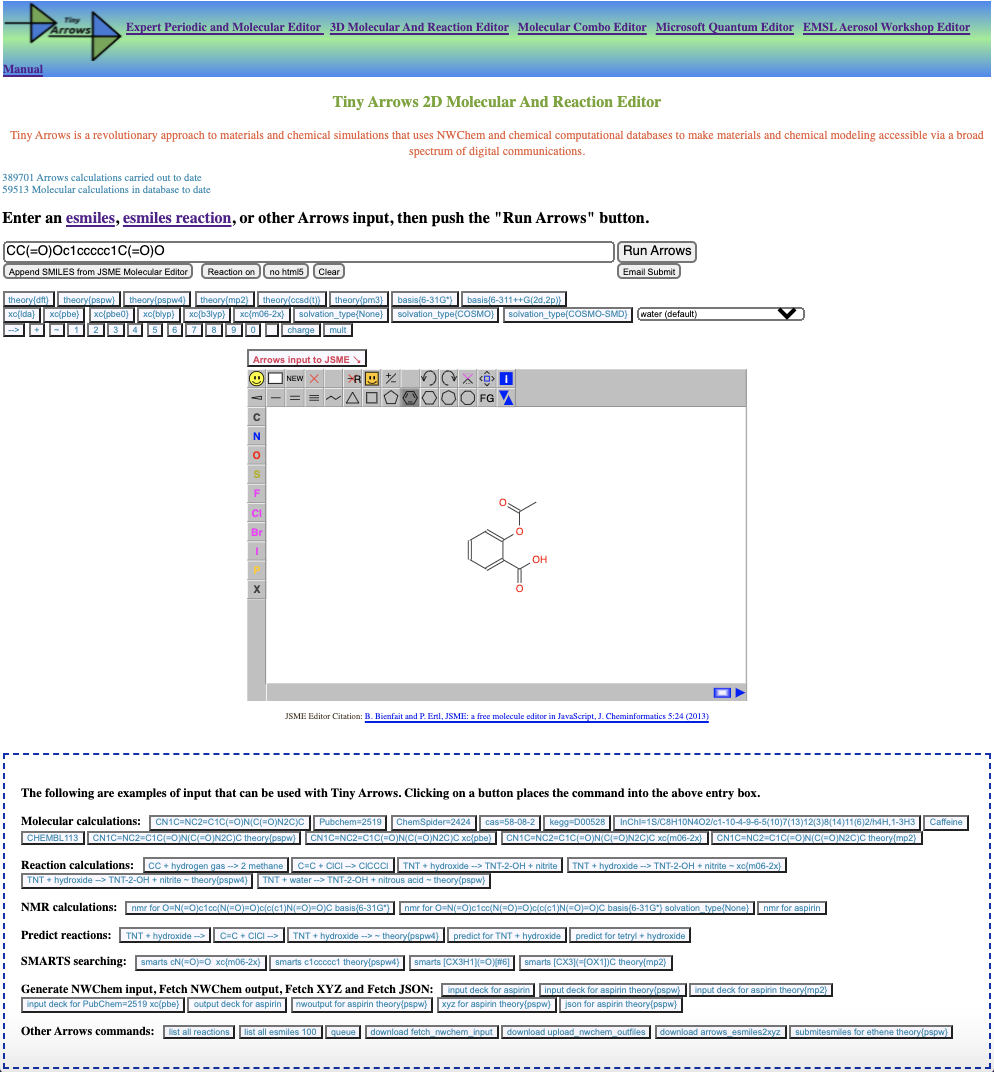
\includegraphics[width=\textwidth]{images/JSME-Input4.png}
   \caption{Snapshot of the basic Arrows web app (\url{http://localhost:5000/api/}).  Below the input bar in the web app, there are several options available that can be used to change the theory, exchange-correlation, basis set, solvation method, charge,  and multiplicity of the \textit{esmiles} and \textit{esmiles reaction} input.  At the bottom of the default Arrows web page, there are examples of commands that can be placed into the entry box.  A JSME molecular editor~\cite{bienfait2013jsme} is integrated into the web-page that can be used to generate SMILES input.  There are also web apps that are integrated with a JSMol molecular builder~\cite{hanson2010jmol,hanson2013jsmol} (e.g., \url{http://localhost:5000/api/3dbuilder}). }
   \label{fig.arrows.input}
\end{figure*}


\begin{figure*}[!h]
   \centering
   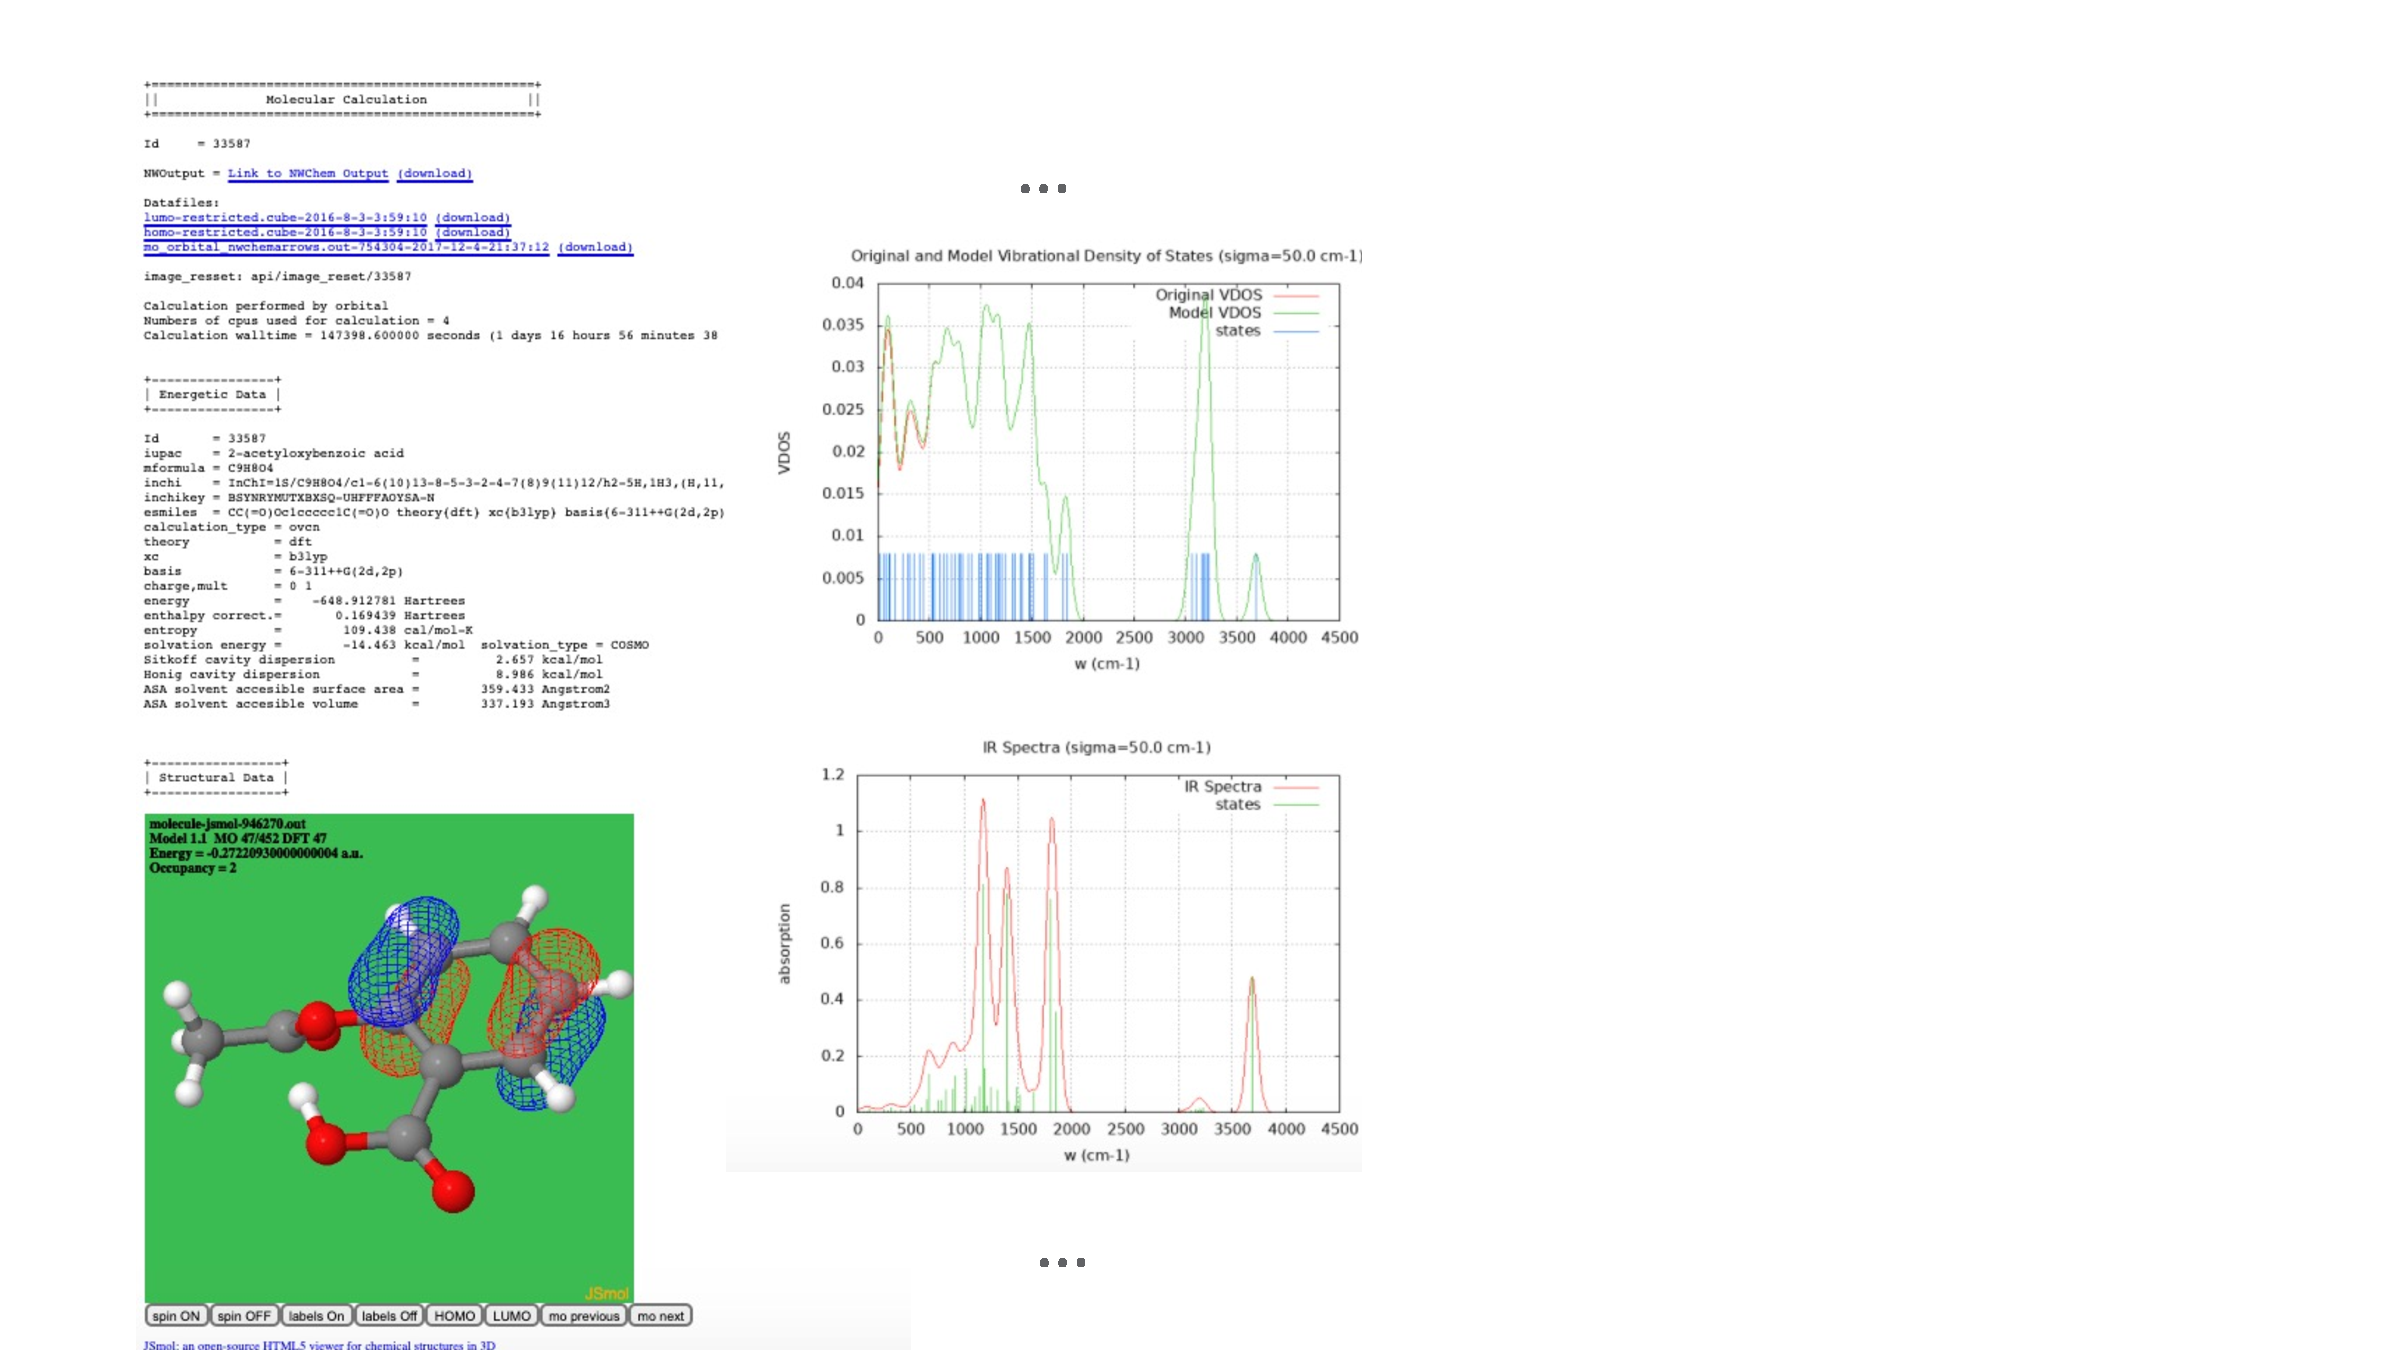
\includegraphics[width=0.9\textwidth]{images/arrows_output2.pdf}
   \caption{Illustration of the output from an Arrows molecular calculation.  The complete molecular output contains sections for "Energetic Data", "Structural Data", "Eigenvalue Data", "Vibrational Density of States Analysis", and "Reactions Contained in the Database" (which contain the molecule). }
   \label{fig.arrows.output}
\end{figure*}

\newpage
The input for a chemical reaction is called an \textit{esmiles reaction} in Arrows.  It is composed of a list of \textit{esmiles} separated by the "\verb|+|" and "\verb|-->|" (dash--dash--greater than) tokens.
To change the calculation options  for an \textit{esmiles reaction} 
 a map function has been added to the reaction input, where the format for the mapping function is to append the reaction with the tilde, "\verb|~|", symbol followed by \verb|keyword{option}| tags.
 Examples of the basic input for chemical reactions are as follows:

\small
\begin{center}
\begin{boxedverbatim}
C(Cl)(Cl)(Cl)O + C  --> C(Cl)(Cl)Cl + CO  
C(Cl)(Cl)(Cl)O + C  --> C(Cl)(Cl)Cl + CO ~ theory{pspw}
C(Cl)(Cl)(Cl)S + C  --> C(Cl)(Cl)Cl + CS
C(Cl)(Cl)(Cl)S + C  --> C(Cl)(Cl)Cl + CS ~ theory{pm3} 
TNT + 3 benzene --> toluene + 3 nitrobenzene ~ xc{pbe} 
cid=8376 + hydroxide --> O=N(=O)c1cc(O)c(c(c1)N(=O)=O)C + nitrite ~ theory{mp2}
carbon tetrachloride + 2 SHE + [H+]  -->  chloroform + chloride 
\end{boxedverbatim}
\end{center}
\normalsize


To run a chemical reaction with Arrows, a chemical reaction (i.e., \textit{esmiles reaction}) is entered as input into the Arrows web app as shown in Fig.~\ref{fig.arrows.rxninput01}, and then the "Run Arrows" input button is selected. 
\begin{figure*}[!H]
   \centering
    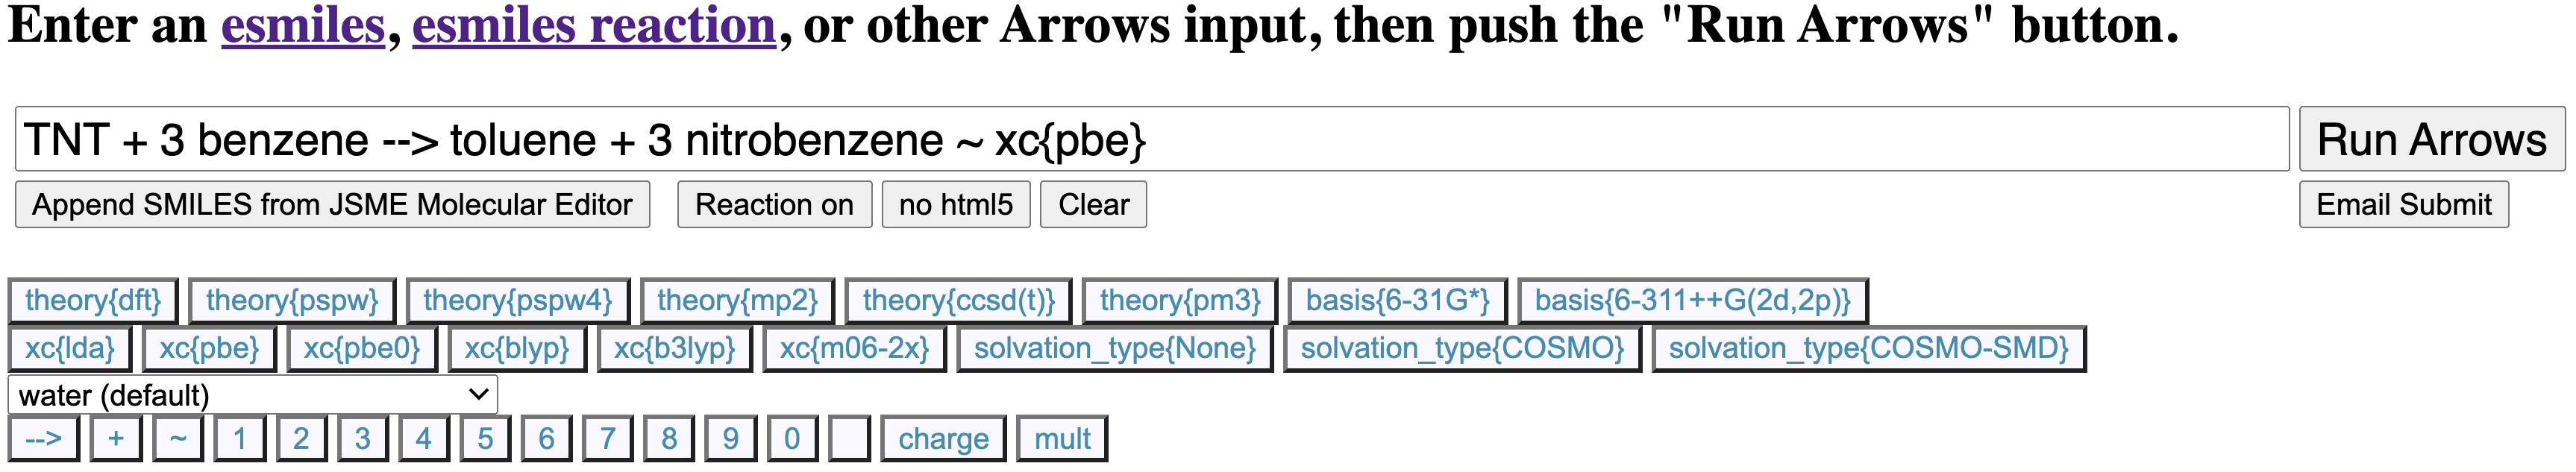
\includegraphics[angle=90,width=0.25\textwidth]{images/rxninput00.png}
   \caption{Example of the basic Arrows input for a chemical reaction (i.e., \textit{esmiles reaction}).  Below the Arrows input, there are several options available that can be used to change the theory, exchange-correlation, basis set, solvation, charge and multiplicity of the \texitit{esmiles} and \textit{esmiles reaction} input.}
   \label{fig.arrows.rxninput01}
\end{figure*}
The results returned by Arrows are a combination of text and graphical output as shown in Fig.~\ref{fig.arrows.rxnoutput01}.

\begin{figure*}[!H]
   \centering
    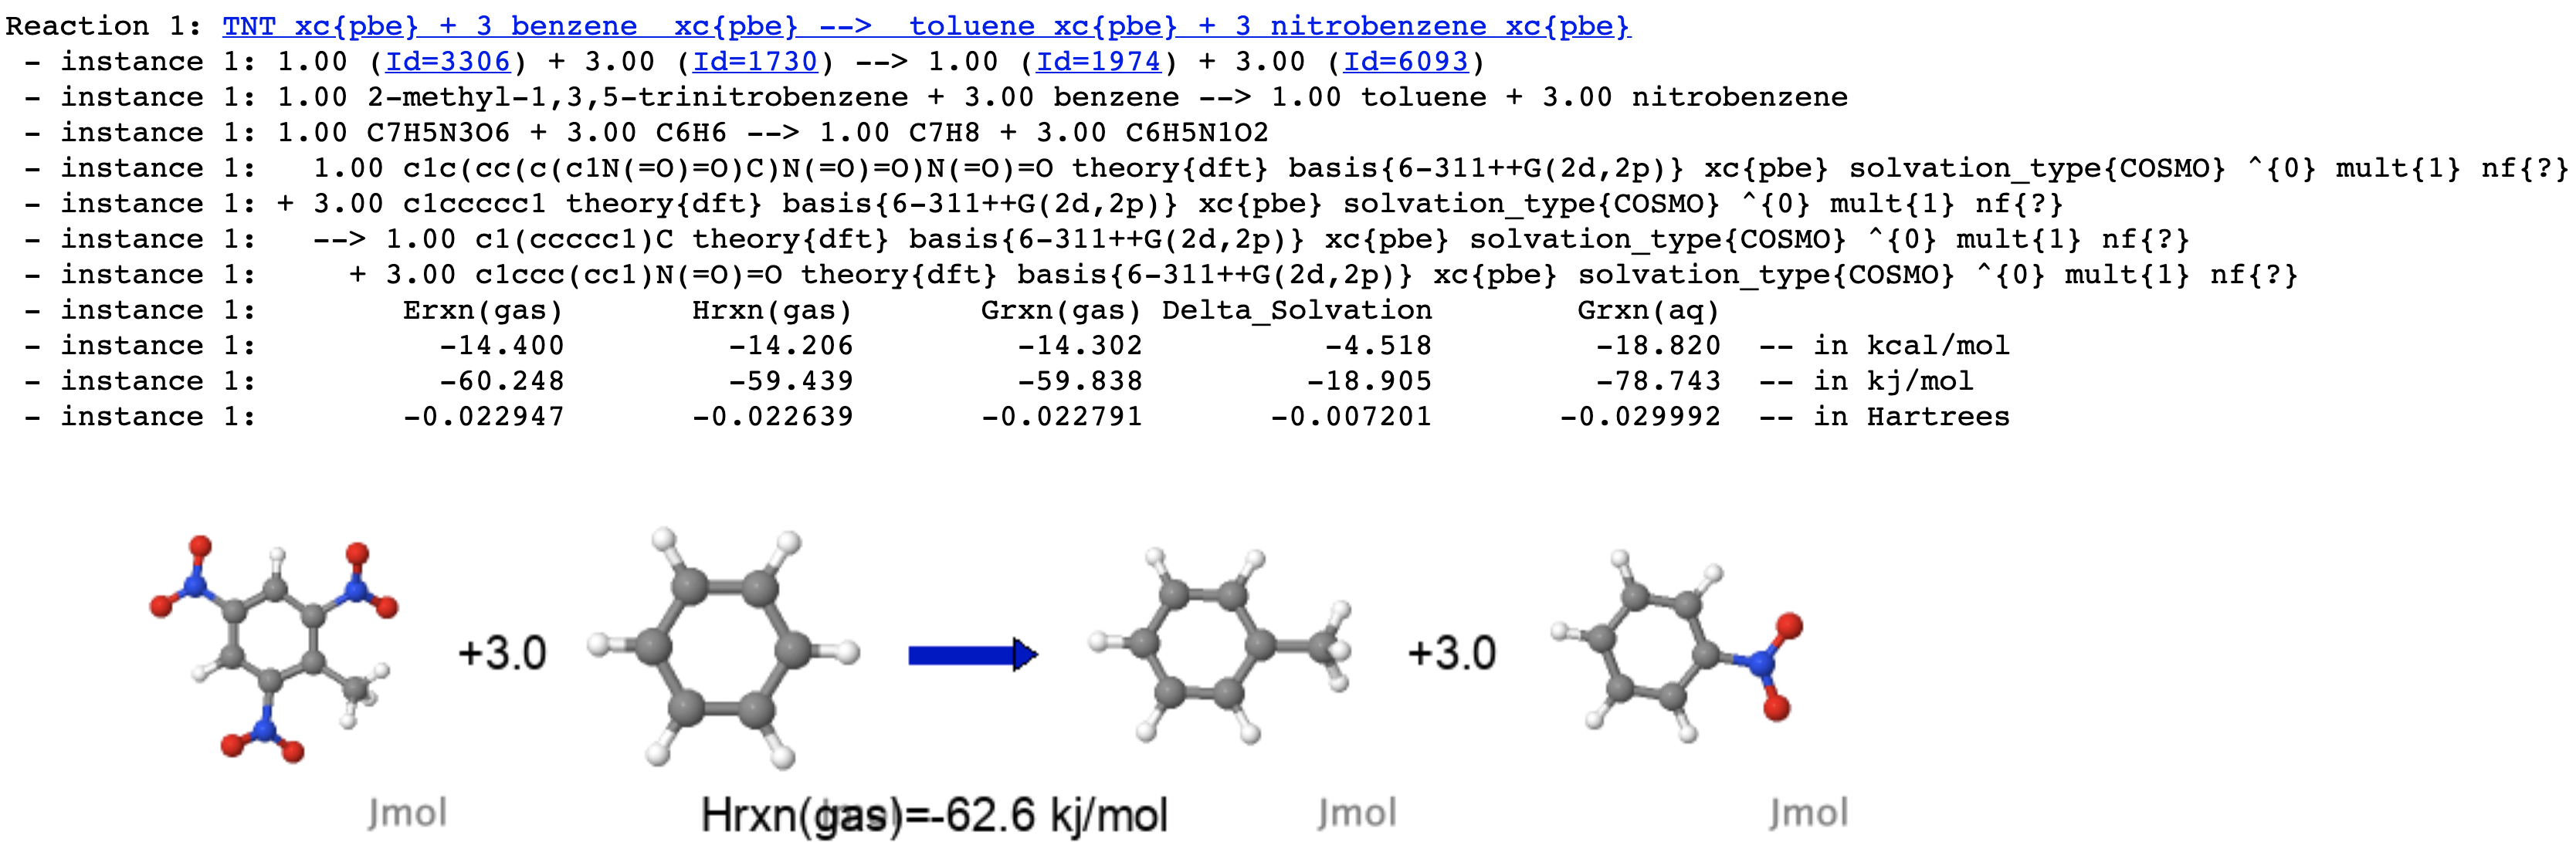
\includegraphics[angle=90,width=0.5\textwidth]{images/rxnoutput01.png}
   \caption{Example of chemical reaction output generated by Arrows using an \textit{esmiles reaction} input. The reaction energy output is given in kcal/mol, kj/mol and Hartree units, and contains the gas-phase energies, enthalpies and free energies of reaction, as well as solvation and aqueous reaction free energies of reaction.}
   \label{fig.arrows.rxnoutput01}
\end{figure*}

\subsection{Other Kinds of Arrows Calculations for More Advanced Computational Scientists}
\label{subsection:otherarrows}
This subsection highlights a variety of other calculations that can be performed with Arrows.  Many of these calculations are designed to be used by expert users of Arrows who have experience in using web services, and who also have expertise in carrying out advanced electronic structure calculations. 

%\begin{figure*}[!h]
%   \centering
%    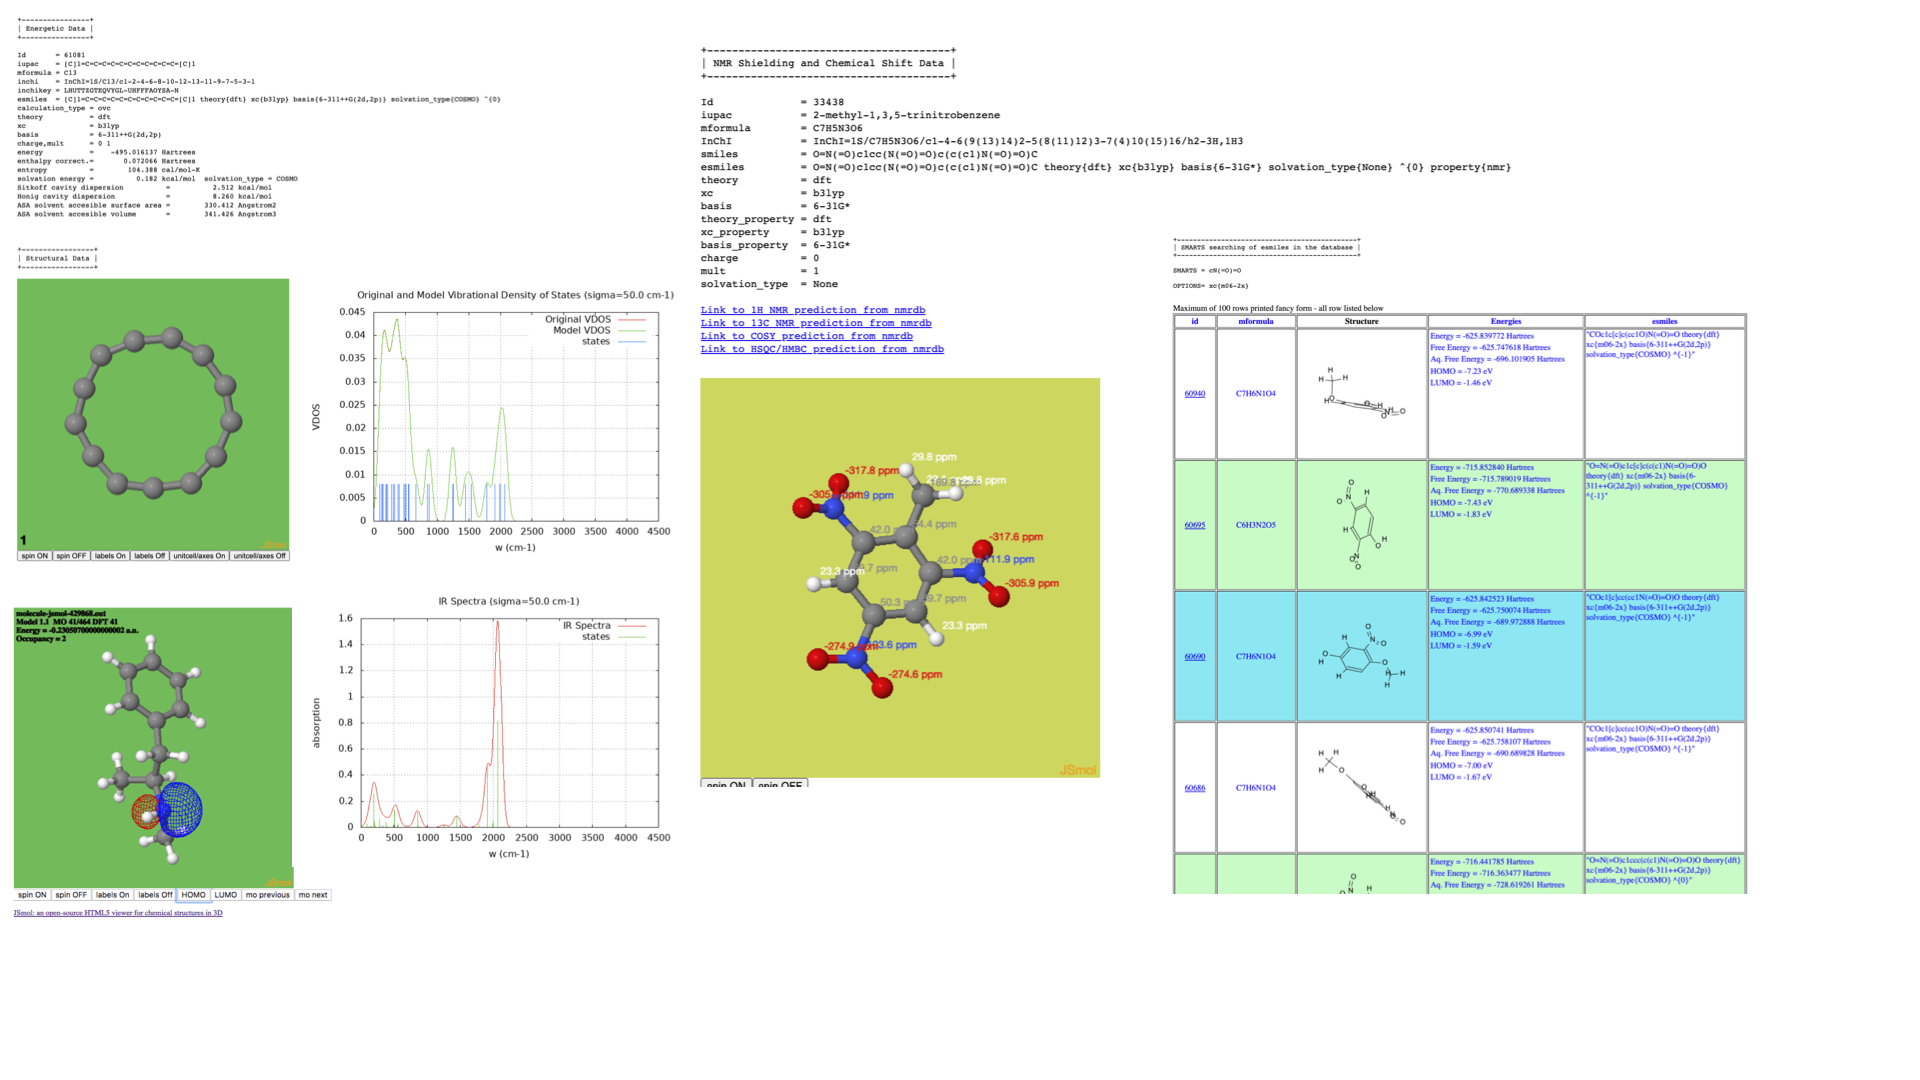
\includegraphics[width=\textwidth]{images/arrowsoutput01.png}
%   \caption{ other caclulations output.}
%   \label{fig.arrows.output02}
%\end{figure*}

\subsubsection{NMR spectra} can be calculated by entering into Arrows an \textit{esmiles} that is preceded by the words “nmr for”, e.g.
\begin{center}
\begin{boxedverbatim}
nmr for c1ccccc1 basis{6-31G*} solvation_type{None}  
\end{boxedverbatim}
\end{center}
\subsubsection{XYZ, JSON, NWChem input, and NWChem output} can be fetched by entering into Arrows an \textit{esmiles} that is preceded by  “xyz for”, "json for", "input deck for", or "output deck for", e.g.
\begin{center}
\begin{boxedverbatim}
xyz for c1ccccc1 basis{6-31G*} 
json for c1ccccc1 basis{6-31G*}
input deck for c1ccccc1 basis{6-31G*}
output deck for c1ccccc1 basis{6-31G*} 
\end{boxedverbatim}
\end{center}
\subsubsection{SMARTS searching} can be performed by entering into Arrows an \textit{esmiles} that is preceded by the words “smarts”, e.g.
\begin{center}
\begin{boxedverbatim}
smarts cN(=O)=O xc{m06-2x} 
smarts c1ccccc1 theory{pspw4}
smarts [CX3H1](=O)[#6]
smarts [CX3](=[OX1])C theory{mp2}
\end{boxedverbatim}
\end{center}
\subsubsection{Input for quantum computing simulations with the Microsoft Quantum Development Kit} - Arrows can be used to generate a Broombridge YAML file containing the 1-electron and 2-electron integrals over a user defined select-CI orbital subspace. This YAML file can be used by the Microsoft Quantum Development Kit chemistry library for quantum chemistry simulations.   The easiest way to generate a Broombridge YAML file is to use Microsoft Quantum Editor web app, which contains a few addition options to help set up the input. The following steps can be used to generate the input and run Arrows.

\noindent\fbox{\parbox{1.0\textwidth}{%
\begin{enumerate}
    \item Press the “Append SMILES from JSME Editor” button to populate the Arrows text box with a SMILES string defined from the structure drawn in the JSME editor~\cite{bienfait2013jsme} to the Arrows input.
    
    \item Press the "filling" button and enter the number of orbitals and electrons. This input defines the orbital subspace. The default filling for qsharp\_chem theory is qsharp\_chem\_filling\{2 1 1\}.
    
    \item Press the "nroots" button and enter the number excited states. The default is to have 0 excited states.
    
    \item Press the basis, charge, and mult buttons to change the basis set, molecular charge and molecular spin multiplicity.
    
    \item Press the "theory{qsharp\_chem}" button to add the Qsharp theory to the Arrows input.
    
    \item Press "Run Arrows"
    
    \item If the data needed to complete the Arrow request is not available, the web-page will contain after the "Link back to Microsoft Quantum Editor" link the text "No molecule data for esmiles". When this happens Arrows will automatically submit a job to one of its calculation queues,
    
    \item If the data to complete the request is available, a link to the YAML file will be available in the "Molecular Calculation" section. The section will look as below.
\end{enumerate}
}}

\begin{verbatim}
...
+==================================================+
||              Molecular Calculation             ||
+==================================================+

Id     = 48414

NWOutput = Link to NWChem Output (download)

Datafiles:
qsharp\_chem.yaml-2018-10-18-13:44:50 (download)

Calculation performed by Eric Bylaska - we29676.emsl.pnl.gov
...
\end{verbatim}
In the Datafiles: subsection click on the (download) link next to the YAML file (e.g. qsharp\_chem.yaml-2018-10-18-13:44:50 in the above example).


\subsubsection{Accessing data using web APIs} - The following restful web APIs that can be used to fetch data from Arrows. The URL formats available are:
\newline

\noindent\fbox{\parbox{1.0\textwidth}{%
\textbf{Restful Web API URL Format:}
\scriptsize 
\begin{itemize}
\item https://arrows.emsl.pnnl.gov/api/molecule/"esmiles parse\_output\{option\}"
\item https://arrows.emsl.pnnl.gov/api/reaction/"esmiles\_reaction parse\_output\{option\}"
\end{itemize} \normalsize
}}
\newline

\noindent where the \textit{esmiles} and \textit{esmiles reaction} input are appended by the parse output option, \verb|parse_output{option}|. The parse output option can be any of the following: \verb|e(gas|), \verb|h(gas)|, \verb|g(gas)|, \verb|g(aq)|, \verb|erxn(gas)|, \verb|hrxn(gas)|, \verb|grxn(gas)|, \verb|grxn(aq)|, \verb|delta_solvation|, \verb|homo|, \verb|lumo|, \verb|alpha_homo|, \verb|alpha_lumo|, \verb|beta_homo|, or \verb|beta_lumo|.  

Here are some examples of calling  restful web APIs in Arrows:
\newline

\noindent\fbox{\parbox{1.0\textwidth}{%
\textbf{Examples of restful Web API URL input:}
\scriptsize 
\begin{itemize}
\item https://arrows.emsl.pnnl.gov/api/molecule/"TNT theory\{pspw4\} parse\_output\{e(gas)\}"

\item https://arrows.emsl.pnnl.gov/api/molecule/"Cl$\backslash$C=C/Cl xc\{pbe0\} parse\_output\{h(gas)\}"

\item https://arrows.emsl.pnnl.gov/api/molecule/"C=CCl xc\{m06-2x\} parse\_output\{g(gas)\}"

\item https://arrows.emsl.pnnl.gov/api/molecule/"TNT theory\{pspw4\} parse\_output\{homo\}"

\item {https://arrows.emsl.pnnl.gov/api/molecule/"TNT parse\_output\{alpha\_homo\}"}

\item https://arrows.emsl.pnnl.gov/api/molecule/"TNT parse\_output\{beta\_homo\}"

\item https://arrows.emsl.pnnl.gov/api/molecule/"DNAN theory\{pspw4\} parse\_output\{lumo\}"

\item https://arrows.emsl.pnnl.gov/api/molecule/"[CH3] \^ \{-1\} parse\_output\{alpha\_lumo\}"

\item https://arrows.emsl.pnnl.gov/api/molecule/"[CH2] mult\{3\} parse\_output\{beta\_lumo\}"

\end{itemize} \normalsize
}}

To use the above APIs, just copy and paste the following lines into web browser URL input, or use with an HTML GET request method in a program written in a programming language such as Python, JavaScript, TypeScript, Java, C\#, C++, Go, Julia, etc..

Unfortunately, the “\#” symbol, which is used to designate a triple bond in a SMILES string, causes problems with URL input.  There are a variety always around this problem. The Arrows APIs have been programmed to use “!” symbol as a replacement for “\#” symbol.  There are also several alternatives to using the "\#" symbol, that can be used in Arrows web API, as listed below.
\newline

\noindent\fbox{\parbox{1.0\textwidth}{%

\textbf{Alternative restful web API URL input for for molecules, such as the ethyne molecule, that use the \# symbol:}

\scriptsize
\begin{itemize}
\item https://arrows.emsl.pnnl.gov/api/molecule/"C!C parse\_output\{h(gas)\}"
\item https://arrows.emsl.pnnl.gov/api/molecule/"HC:hash:CH parse\_output\{h(gas)\}"
\item https://arrows.emsl.pnnl.gov/api/molecule/"HC&num;CH parse\_output\{h(gas)\}"
\item https://arrows.emsl.pnnl.gov/api/molecule/"[H][C][C][H] parse\_output\{h(gas)\}"
\item https://arrows.emsl.pnnl.gov/api/molecule/"InChI=1S/C2H2/c1-2/h1-2H parse\_output\{h(gas)\}"
\item https://arrows.emsl.pnnl.gov/api/molecule/"acetylene parse\_output\{h(gas)\}"
\item https://arrows.emsl.pnnl.gov/api/molecule/"pubchem=6326 parse\_output\{h(gas)\}"
\item https://arrows.emsl.pnnl.gov/api/molecule/"kegg=C01548  parse\_output\{h(gas)\}"
\item https://arrows.emsl.pnnl.gov/api/molecule/"cas=74-86-2  parse\_output\{h(gas)\}"
\item https://arrows.emsl.pnnl.gov/api/molecule/"chemspider=6086 parse\_output\{h(gas)\}"
\item https://arrows.emsl.pnnl.gov/api/molecule/"CHEMBL116336 parse\_output\{h(gas)\}"
\end{itemize}
\normalsize
}}
\newline

Using these web APIs, one can fetch data from Arrows directly into Google sheets (UrlFetchApp script) and Microsoft Excel (Windows version only) spreadsheets using scripting (i.e. the UrlFetchApp in Google sheets, and the fetch API in Excel).
\begin{figure*}[!H]
   \centering
    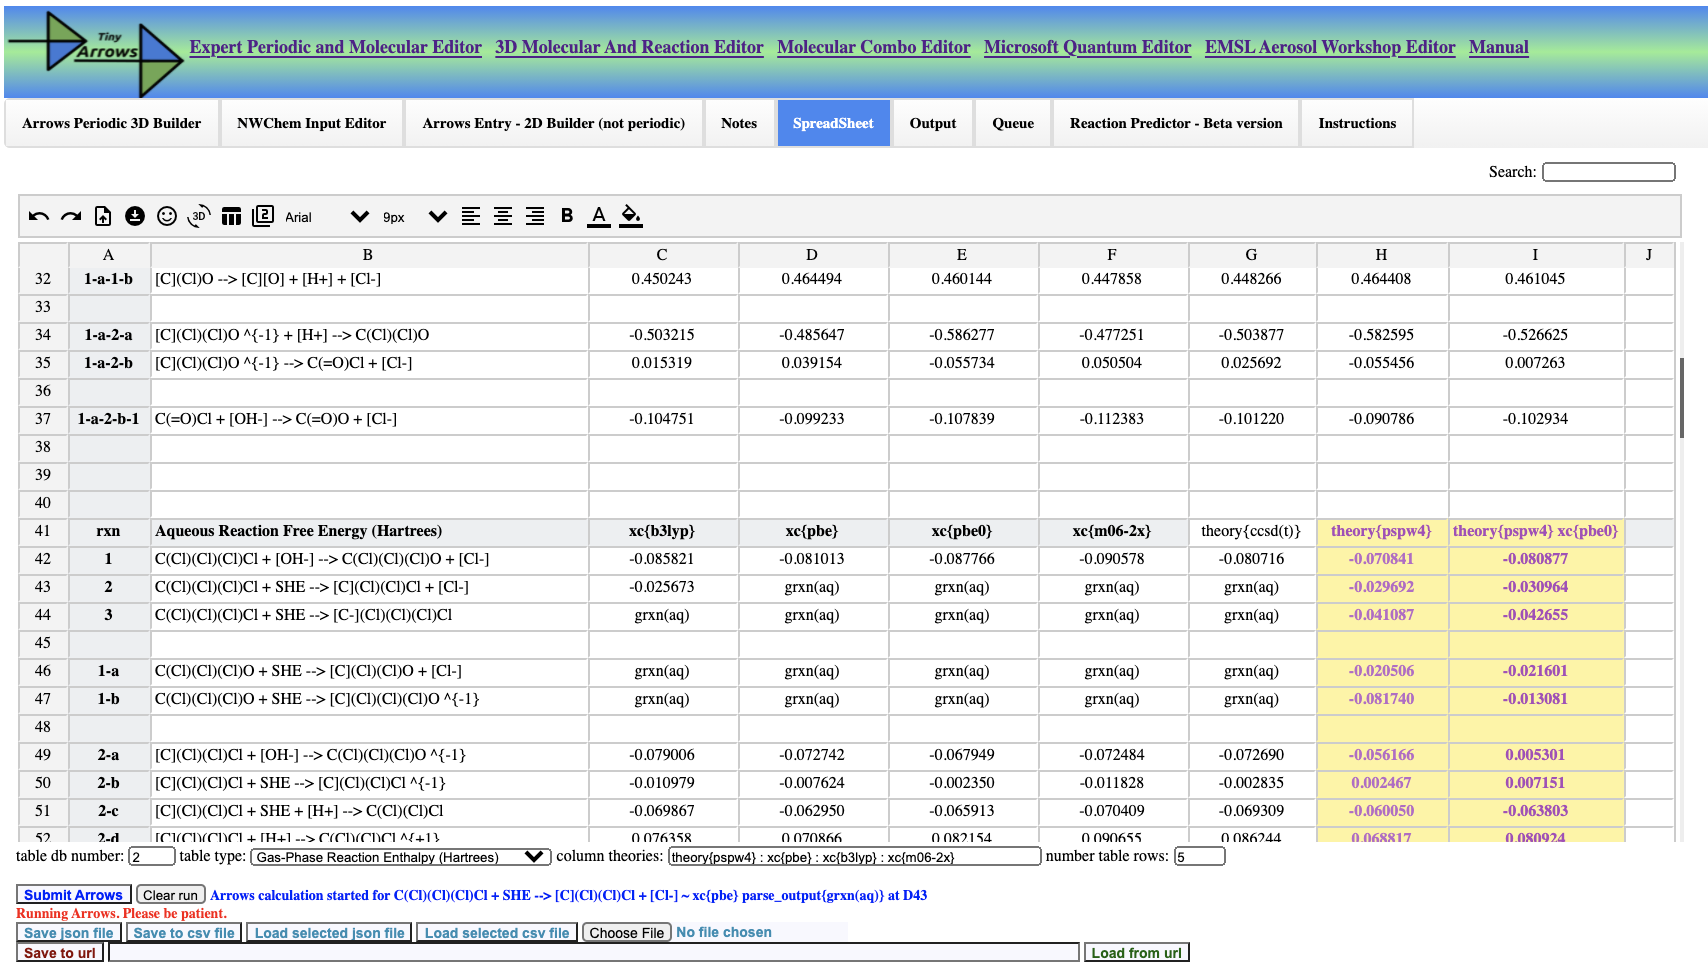
\includegraphics[angle=90,width=0.9\textwidth]{images/arrows_spreadsheet.png}
   \caption{Illustration of using the Arrows spreadsheet capability to calculate reaction energies for the reactions contained in the CCl$_4$ reaction network illustrated in Fig.~\ref{fig.enviro.ccl4network} (vida infra).}
   \label{fig.arrows.spreadsheet}
\end{figure*}
\subsubsection{SpreadSheet Input} - There is also a spreadsheet capability, Jspreadsheet~\cite{JSspreadsheet}, that has been integrated in Arrows as shown in Fig.~\ref{fig.arrows.spreadsheet}.  To use it, navigate to the "Expert Periodic and Molecular Editor" web app, and then select the "SpreadSheet" tab.  The following steps can be used to make a table in the spreadsheet that can filled in with calculations from Arrows:

\noindent\fbox{\parbox{0.95\textwidth}{%
\textbf{Using Spreadsheet to Create an Arrows Calculation Table:}
\begin{enumerate}
    \item  Just below the spreadsheet,  select a table type from the list of table types (e.g., "Gas-Phase Reaction Enthalpy (Hartrees)"). 
    
    \item To right the right of the table type input, enter \textit{esmiles} options, separated by ":", in the column theory input.
    
    \item In the next input to the right enter the number of table rows, which is the number of \textit{esmiles} or \textit{esmiles reaction} that will be calculated. 
    
    \item Once these inputs are set, select a cell in the spreadsheet where to place a table template.  To place the template, select the table icon (7th icon from the right) in the options at the top of the spreadsheet.  
    
    \item To complete the table input, enter \textit{esmiles} or \textit{esmiles reaction} as the row labels, replacing the row labels temporarily filled in with the \textit{esmiles} or \textit{esmiles reaction} string.  Note, the smiley face icon can be used to place a smiles string for the structure currently residing in the  2D builder tab.
    
    \item To fill in the body of the table with values calculated from Arrows, just select the "Submit Arrows" button below the spreadsheet.
\end{enumerate}
}}

\subsubsection{The Arrows Queues} are used to manage NWChem and other jobs on machines that have HTTP access to a running Arrows web service.  
There are two queues in Arrows.  The standard queue in Arrows, called "queue", is used to keep track of NWChem calculations that were generated when a request was made for a compound that was not available in the Arrows databases.  The jobs on the queue can be obtained by entering "queue" in the Arrows input.  In addition, to the standard queue in Arrows, there is also a second queue, called "queue\_nwchem", that can be used to manage user specified NWChem (and other program) input and output decks. A list of jobs on the queue\_nwchem can be obtained by entering "queue\_nwchem" in the Arrows input. The two Arrows queues can also be accessed using the following URLs.

\noindent\fbox{\parbox{0.95\textwidth}{%
\textbf{URL commands to list jobs on the queue and nwchem\_queue:}
\begin{itemize}
\item \url{https://localhost:5000/api/queue} [GET]
\item \url{https://localhost:5000/api/queue_html} [GET]
\item \url{https://localhost:5000/api/queue_nwchem} [GET]
\item \url{https://localhost:5000/api/queue_nwchem_html} [GET]
\end{itemize}

\textbf{URL commands to fetch and delete from from the queue and nwchem\_queue:}
\begin{itemize}
\item \url{https://localhost:5000/api/queue_fetch/<id>} [GET]
\item \url{https://localhost:5000/api/queue_nwchem_fetch/<id>} [GET]
\item \url{https://localhost:5000/api/queue_delete/<id>} [GET]
\item \url{https://localhost:5000/api/queue_nwchem_delete/<id>} [GET]
\end{itemize}

\textbf{URL commands to upload jobs to the queue and nwchem\_queue}
\begin{itemize}
\item \url{https://localhost:5000/api/upload/} [POST:files]
\item \url{https://localhost:5000/api/submit_output} [GET]
\item \url{https://localhost:5000/api/submit_nwchem_output} [GET]
\end{itemize}
}}

\subsubsection{The Advanced Builders Implemented in Arrows}
can also be used to carry out computational chemistry and other electronic structure calculations using its more traditional web-based periodic and molecular builders.  These builders are written in JavaScript, and they contain the following capabilities:

\noindent\fbox{\parbox{1.0\textwidth}{%
\textbf{Periodic and Molecular Builder Web Applications Implemented in Arrows:}
\begin{enumerate}
    \item Works on any web browser on workstations, laptops, tablets, smart phones.
    \item Extensive options to build and modify periodic and cluster systems. 
    \item Create, edit, load and save NWChem input decks and submit jobs.
    \item Generates and cleaves surfaces in seconds.
    \item Options for setting up initial reaction pathways, free energy simulations, electron transfer calculations.
    \item Space-group symmetry.
    \item Text and spreadsheet editors.
    \item MM optimization.
    \item Solvation for periodic systems via web API.
    \item Workflows to carry out various reaction pathway/TST methods including 
    \begin{itemize}
        \item NEB method
        \item WHAM reaction free energy with Hausdorff moments fitting of histograms
        \item String method, 
        \item Reaction coordinate penalty functions (e.g. $E_{\mathrm{penalty}}=\frac{K}{2}(\gamma({R_I})-\gamma_0)^2$ where $\gamma({R_I})$ is the order parameter or collective variable of the reaction and $\gamma_0$ is a constant), 
        \item Potential of mean force,
        \item  WHAM reaction free energy with Hausdorff moments fitting of histograms
        \item Metadynamics,
        \item TAMD,
        \item Single sweep AIMD free energy methods,
    \end{itemize}
    \item AIMD-EXAFS workflow.
    \item User defined workflows through the use of a scripting language implemented directly in the advanced builders.
    \item Reaction prediction.
    \item View NWChem output, structures, trajectories, Gaussian cube files, free-energy surfaces, etc.
\end{enumerate}
}}

\subsubsection{Predicting Reaction Pathways} - 
A variety of chemical reaction pathway prediction toolboxes have become available in recent years~\cite{pensak1977lhasa,karp2002pathway,socorro2005robia,yang2017automatic,stocker2020machine,gao2016reaction,doi:10.1021/acs.energyfuels.0c03843,rappoport2019predicting}.  The development of rules-based systems like LHASA~\cite{pensak1977lhasa}, EPA-CTS~\cite{wolfe2016chemical} (\url{https://www.epa.gov/cts/}) and EAWAG-BBD~\cite{wicker2010predicting} (\url{http://eawag-bbd.ethz.ch/predict/}), KinBot~\cite{zador2013kinbot,van2020kinbot}, RMG~\cite{suleimanov2015automated}, and IBM RXN for Chemistry(\url{https://rxn.res.ibm.com/}) ultimately can provide a universal solution to path pathway prediction.  However, these methods require lots of input and detailed knowledge of the chemistries being modeled.  As a result, these developments have been spanning over decades, even though the underlying computing hardware needed to run these methods is not changing.  Another approach for pathway prediction is to use brute force combinatorics, which generate possible reaction mechanisms with electronic structure calculations to evaluate the reaction pathways. These methods break N bonds and make M bonds, where M and N are defined to be relatively small to limit the number of results. Because of the large number of products produced even with M,N< 4, these approaches need to be augmented with quick energetic filters such as classical molecular dynamics potentials, machine-learning potentials, and Benson group methods~\cite{suleimanov2015automated}. 

\begin{figure*}[!H]
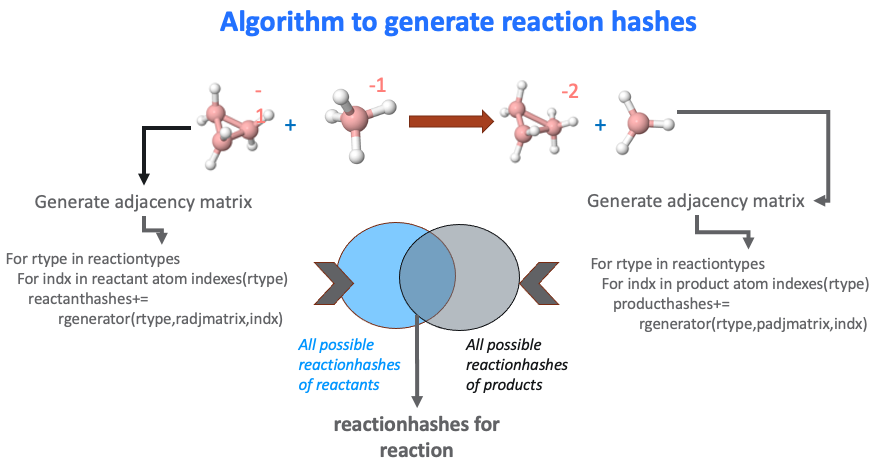
\includegraphics[angle=90,width=0.8\textwidth]{images/gerhash.png}
\caption{Illustration of algorithm to generate a reaction hash from a balanced chemical reaction.}
\label{fig.arrows.reactionhashes}
\end{figure*}

We have been developing an alternative learning approach for predicting reactions in Arrows using predicate calculus learning~\cite{Charniak1985} based on defining canonical reaction hashes.  Reaction hashes classify reactions by defining the connectivity of the atoms relative to a reaction coordinate. The hashes generated in this way can be quite big for larger systems, however, they can easily be made more manageable by restricting how far the connectivity is spanned.  Given the adjacency matrix of a chemical system (where the XYZ coordinates of reactants or products of a reaction can be used to define an adjacency matrix), a reaction hash is created by specifying the type of reaction (e.g., \verb|A + B --> AB|, \verb|AB + C --> AC + B|, \verb|AB + CD --> AC + BD|, \verb|EA + BCD --> AB + CDE|, ...) and the indexes of atoms involved in the reaction coordinate.  In other words, a hash function is defined in Arrows that generates a hash string
\small
\begin{equation*}
    \textit{hash string} = \textbf{ReactionHash}(\textit{XYZ string},\text{"2 1 8"}, \text{"AB + C --> AC + B"}) ,
\end{equation*}
\normalsize
that contains information about the connectivity of the chemical system, where the three input strings describe the XYZ coordinates for the reactants, atom indexes (e.g. "2 1 8"), and the reaction type (e.g. \verb|"AB + C --> AC + B"|).

\begin{figure*}[!H]
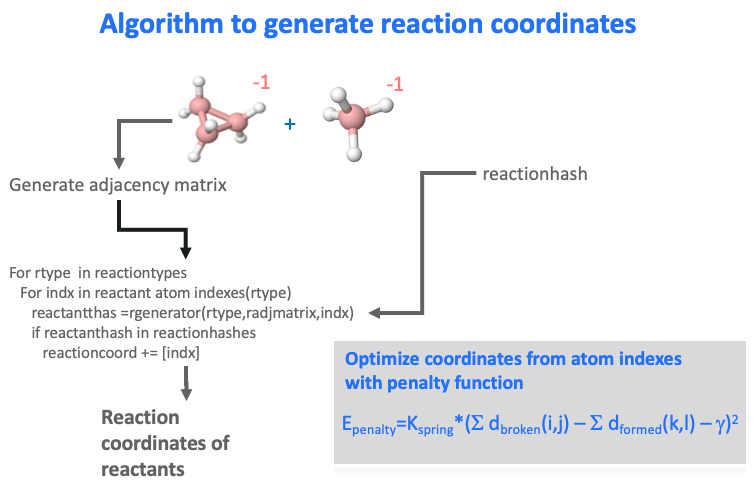
\includegraphics[angle=90,width=0.8\textwidth]{images/gencoords.png}
\caption{Illustration of algorithm to generate reaction coordinates given a reaction hash and reactants.}
\label{fig.arrows.reactionhashes2}
\end{figure*}
Using these hash functions, canonical reaction hashes for a balanced chemical reaction can be generated using the algorithm illustrated in Fig.~\ref{fig.arrows.reactionhashes}.  These canonical hashes can be used to find products given the reactants, and to define initial reaction pathways for Nudged Elastic Band (NEB)~\cite{jonsson1998nudged,henkelman2000climbing}, and string calculations~\cite{weinan2002string}.  By making a database of reaction hashes from a set of balanced chemical reactions, it is possible to generate future chemical reactions by filtering the hash to reduce how far it spans the chemical graph (Fig.~\ref{fig.arrows.reactionhashes2}).  Both the initial reaction pathway and reaction learning capabilities are available in Arrows.
\begin{itemize}
\item Initial reaction pathways can be generated using the web-based periodic and molecular builders web application by selecting the "reaction input" in the "Arrows Periodic 3D Builder" tab.  
\item Reaction predictions can be calculated by using the "Reaction Predictor - (Beta Version)" tab in the web-based periodic and molecular builders" web application, or by 
entering into the Arrows input (or using the reaction web api) only the reactants of an \textit{esmiles reaction} followed by the reaction arrow "\verb|-->|", e.g.,
\end{itemize}
\begin{center}\begin{boxedverbatim}
C=C + ClCl -->  
TNT + hydroxide --> 
TNT + hydroxide --> ~ theory{pspw4}
DNAN + [SH-] -->  
\end{boxedverbatim}
\end{center}


\section{Applications}
\label{sec:Applications}
Arrows or early versions of capabilities in the Arrows have been used to carry out a variety of scientific studies~\cite{salter2015predicting,bylaska2017plane,bylaska2019association,low2019q,north2020nitrogenase,torralba2020reduction,trainer2020organic,mcneill2020reaction,bylaska2020filon,ilton2020using,harouaka2020gas,bylaska2020electron,apra2020nwchem,bylaska2021quantum,mergelsberg2021resolving,gao2021quantitative}. Most of these studies fall into two categories.  The first use cases are for performing large numbers of molecular and reaction energy calculations.  The second use cases employ the workflow capabilities in Arrows to carry out complex simulations, e.g. ab initio molecular dynamics informed extended X-ray absorption fine structure (AIMD-EXAFS~\cite{fulton2012near}), and hybrid AIMD and molecular dynamics (AIMD/MM~\cite{laio2002hamiltonian,cauet2010structure}) free energy simulations.  

The following subsections highlight using Arrows to carry out molecular computations in two areas of the authors' research: environmental chemistry and materials computations for geochemistry (and catalytic chemistry). 


\subsection{AIMD Simulations and Workflows in Geochemistry and Catalysis}
\label{sec:geochemistry}

The interpretation of geochemical and related catalytic surface processes are complicated by chemical complexity and structural heterogeneity of natural materials and their interfaces, as well as by the wide range of temperature and pressure conditions under which they occur. Unraveling the nature of these processes in terms of key molecular-level reactions under realistic conditions is a grand challenge in geochemistry and catalysis. AIMD simulations are well suited to make inroads in this area of chemistry~\cite{swaddle2005kinetic,rustad2007ab,atta2012structure,fulton2012near,solve1,solve2,rustad2010isotopic,rustad2010calculation,bylaska2007structure,nichols2008equatorial,cauet2010structure,bogatko2010first,bogatko2013aqueous,mcbriarty2017trace,mcbriarty2017dynamic,kerisit2016ab,bylaska2019association,bylaska2020filon,ilton2020using}.

In recent years,  Bylaska and collaborators have demonstrated that AIMD simulations can provide accurate hydration structures for a series of divalent and trivalent dissolved cations (Al$^{3+}$, Ca$^{2+}$, Cr$^{3+}$, Mn$^{2+}$, Fe$^{3+}$, Co$^{2+}$, Ni$^{2+}$, and Zn$^{2+}$) that yields near-quantitative agreement with their EXAFS spectra~\cite{bylaska2007structure,fulton2012near,bogatko2010first,bogatko2013aqueous}.  The AIMD-EXAFS~\cite{fulton2012near,nichols2008equatorial} method has been applied to several systems including the U$^{4+}$, U$^{5+}$, U$^{6+}$, and Cm$^{3+}$ aqueous species~\cite{atta2012structure,solve2,atta2011hydration}. Bylaska and Ilton recently used the AIMD-EXAFS approach to study U(IV), U(V), and U(VI) substitution into goethite, hematite, and lepidocrocite and the associated defects~\cite{kerisit2016ab,mcbriarty2017trace,mcbriarty2018iron,ilton2020using}.


\begin{figure*}[!H]
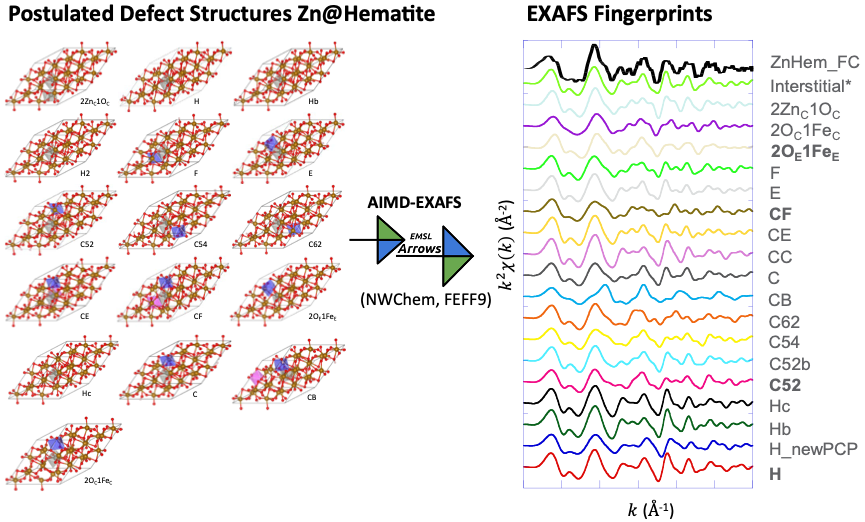
\includegraphics[angle=90,width=0.9\textwidth]{images/AIMD-EXAFS.png}
\caption{The simulated EXAFS spectra for 16 possible defect structures of Zn in hematite, excluding a structure for the interstitial site.  Note H\_newPCP and H are same structure, but spectra was calculated using different pseudopotentials.}
\label{fig.app.aimd-exafs}
\end{figure*}


The AIMD-EXAFS approach was recently extended to characterize the composition and structure of  Zn(II) and Cu(II) point defects in hematite~\cite{bylaska2019association,mergelsberg2021resolving} (see Fig.~\ref{fig.app.aimd-exafs}). Point defects play an important role in the physics and chemistry of materials including ionic conductivity, diffusion, general reactivity, creep, optical behavior, radiation damage, and many other phenomena. They also play a critical role in regulating the fate and transport of minor yet critical metals, including micronutrients and contaminants, in the environment.  For example, at normal background concentrations, Zn(II) is an essential nutrient.  However, due to anthropogenic activities, it can be released in large enough concentrations that it can exhibit high levels of toxicity.  A salient point is that the potential incorporation of Zn in secondary refractory minerals such as Fe(III) (oxyhydr)oxides can decrease bioavailable Zn below levels indicated by measured total concentrations.  

It was previously predicted by Catalano et al. that Zn was immobilized as a tetrahedral coordinated defect in hematite. The predicted structure of this defect was based on EXAFS using a traditional shell by shell fitting procedure.  The authors noted that the tetrahedral coordination of Zn in hematite was problematic, as the distances and CN to second-nearest neighbor Fe$^{3+}$ atoms were consistent with Zn substituting for Fe$^{3+}$ in regular octahedral sites.  Furthermore, the
Debye-Waller factor for first shell Zn-O in hematite was unusually  high.  This suggested possible unresolved configurational disorder. 

In order to resolve these inconsistencies, the fitting of the experimental EXAFS spectra was revisited using an AIMD-EXAFS approach.  In contrast to the earlier work, these follow-on studies, which produced fittings with reasonable Debye-Waller factors, indicated the presence of three configurations that were dominated by octahedral coordination.

While AIMD-EXAFS simulations have proven to be useful, and they do not have the limitations of shell-by-shell fitting that (often) leads to simplifying assumptions, they are difficult and time-consuming to carry out. They require setting up and running multiple different AIMD simulations of large unit cells containing defects with specified spin and charge configurations, running thousands of FEFF calculations per trajectory, Fourier transforming and averaging the spectra from each trajectory, and finally comparing the experimental spectra with linear combinations of the calculated fingerprint spectra to extract likely structures.  Moreover, depending on the size of the unit cell, each AIMD simulation may need to be run in stages for the AIMD trajectory to be long enough (e.g. each AIMD simulation is restarted 25 times). The following workflow details the steps used to carry out the AIMD-EXAFS simulations of the Zn(II) and Cu(II) in hematite.
\newline

\noindent\fbox{\parbox{1.0\textwidth}{%
\textbf{AIMD-EXAFS Workflow Using Arrows:}
\begin{enumerate}
    \item Create the unit cell with a defect, set up the AIMD simulation, and submit to the Arrows queue. 
    \item If using TinyArrows, SSH with port forwarding to a computer center from a machine running the TinyArrows web server.
    \item At the external computer center:
    \begin{itemize}
       \item Fetch the AIMD job from the Arrows queue and submit the job to the computer center's queue.
       \item When the simulation is finished, upload simulation results to the Arrows queue. (When uploaded, the Arrows queue processes the results and automatically submits a restart job if more simulation time is needed).
       \item Repeat until there are no more jobs on Arrows queue
    \end{itemize}
    
    \item Fetch the trajectory data from the Arrows queue to a local workstation.
    \item Parse the trajectory and submit 1000s of EXAFS (FEFF) jobs to the Arrows queue.
    \item These jobs are then fetched, run with EXAFS calculations, and results uploaded using available workstations.
    \item EXAFS results on the Arrows queue are then collated and averaged into fingerprint spectra for use in analysis of experimental spectra.
 \end{enumerate}
}}
\newline

This workflow, which heavily utilizes the Arrows queue to move data between different computer systems, was implemented with Python scripts running as cron jobs on various machines.  These scripts just run through a simple cycle of repeated steps: (i) List the Arrows queue (arrows\_queue\_nwchem\_get\_url), (ii) Download an input deck from arrows queue (arrows\_queue\_fetch\_get\_url), (iii) Run the input deck, (iv) Upload the output deck to the Arrows queue (arrows\_post\_url), (v) Submit the output (arrows\_submit\_output\_get\_url), and go to (i).  Access to the Arrows queue in above workflow and its associated scripts used the HTTPS GET and POST requests described in Arrows Queue subsection in section~\ref{subsection:otherarrows}.  Once the workflow is started, all the succeeding steps were done automatically.



\subsection{New insight into Environmental Reactions Using Chemical Reaction Networks}
\label{subsection:enviro}

As illustrated previously in Fig.~\ref{fig.intro.rxnnetwork}, the degradation of many pollutants in natural ground-waters will involve large reaction networks consisting of numerous reaction pathways.  Obtaining all the parameters needed from experimental measurements, while hypothetically possible, would end up being time-consuming and not practical for most systems. Even with computation, this can become an arduous task.  In this subsection, we demonstrate how Arrows can be used to map out possible reaction pathways for the degradation of a prototypical pollutant, CCl$_4$. 

\begin{figure*}[!H]
   \centering
   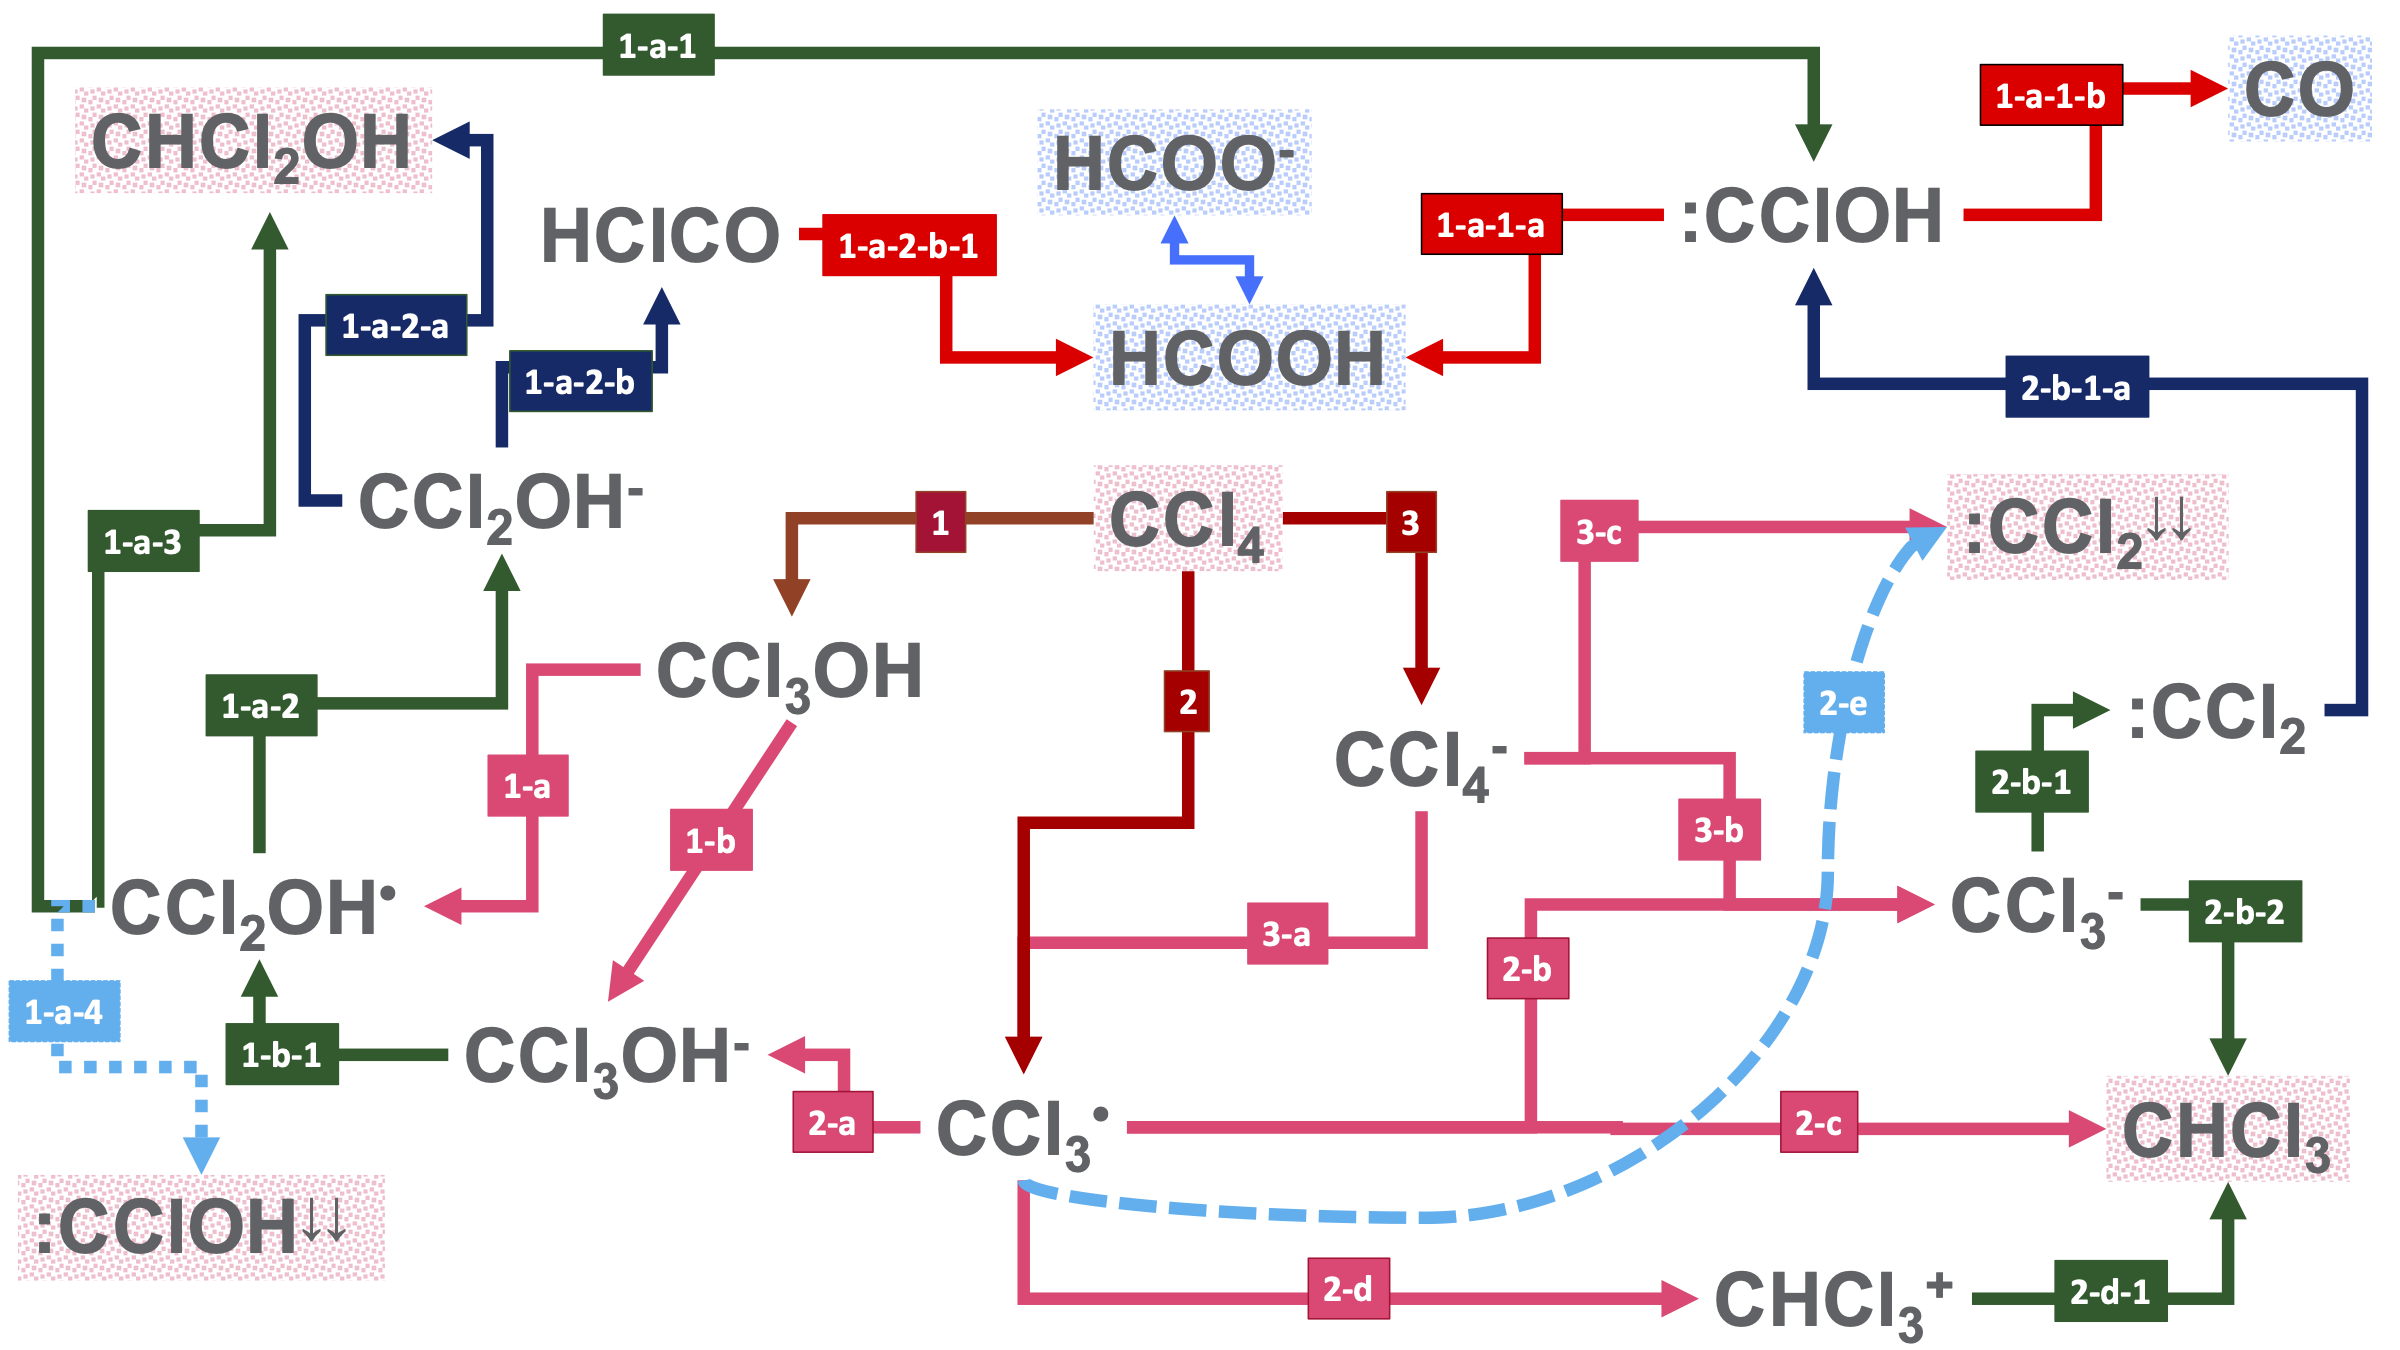
\includegraphics[angle=90,width=0.8\textwidth]{images/CCl4networks2.png}
   \caption{Hypothesized reaction network for the degradation of CCl$_4$ in the environment under reducing conditions.}
   \label{fig.enviro.ccl4network}
\end{figure*}


Over the years several groups have used the standard tools of quantum chemistry, to estimate the thermodynamics and kinetics of the possible degradation reactions for CCl$_4$ with a variety of theories and methods, including high-level electronic structure and DFT~\cite{hohenberg1964inhomogeneous,kohn1965self} methods, QM/MM and continuum solvent models, and advanced free energy methods~\cite{kumaran1996ab,bylaska2000free,borisov2001systematic,bylaska2002one,bylaska2006estimating,valiev2008combined,feller2001extended,feller2003performance,chen2013water,robertson2002solvation,wang2012hybrid,koper1998theory,saveant1987simple,camaioni2009modeling}. Despite the extensive literature using electronic structure methods to model CCl$_4$, these studies were primarily focused on individual reactions or particular classes of reactions, rather than considering the reaction network as a whole. An advantage of Arrows is that it becomes feasible to study reaction networks in their entirety.  

For example, one of the motivations of this work has been the "chlorform problem" in which it has been suggested there are competing reaction pathways for the degradation of CCl$_4$ that can produce unfavorable and favorable metabolites~\cite{tratnyek1998situ,national1978chloroform,pankow1996dense,truex2001assessment,amonette2000dechlorination,kriegman1994transformation,kriegman1992transformation,pecher2002reduction,assaf1994reduction,krone1991reductive}.  Unfortunately, many groundwater remediation strategies follow an unfavorable pathway in which they produce  chloroform (CHCl$_3$) as the major product and methylene chloride (CH$_2$Cl$_2$) as a minor product. Both of these products are nearly as persistent and problematic as the parent compound, but there are competing reaction pathways that could produce more desirable products, carbon monoxide (CO) and/or formic acid (HCOOH).  Results scattered throughout the chemical and environmental engineering literature have suggested the branching between these reaction pathways is highly variable, but the controlling factors have not been identified. 

In Fig.~\ref{fig.enviro.ccl4network}, a hypothesized reaction network, containing 27 elementary reduction and hydrolysis steps, is shown for the first few steps of CCl$_4$ degradation.  This network was designed to capture common elements in the degradation of CCl$_4$, regardless of whether it occurs as an intracellular metabolic process, an enzyme-catalyzed process in vitro, an abiotic reaction catalyzed on mineral surfaces, or even an electrode reaction. If we understood the fundamental chemistry that controls the branching among these, and related, product-formation pathways, we could improve the applicability of a host of remediation technologies (both chemical and biological) to the large plumes of CCl$_4$ that contaminate DOE sites across the country. 
\subsubsection{Thermodynamic calculations} for the hypothesized reactions in solution are given in Table~\ref{tab:ccl4rxn}.  Seven different electronic structure methods were used to carry out the calculations, including four DFT~\cite{hohenberg1964inhomogeneous,kohn1965self} calculations using B3LYP~\cite{beck1993density,lee1988development}, PBE~\cite{perdew1996generalized}, PBE0~\cite{adamo1999toward}, and M06-2x~\cite{zhao2008m06} exchange-correlation functionals with the 6-311++G(2d,2p)~\cite{clark1983a,francl1982a,krishnan1980a,mclean1980a,spitznagel1987a} Gaussian basis set, two plane-wave DFT calculations with PBE and PBE0 exchange-correlation functionals, and frozen core CCSD(T)/6-311++G(2d,2p) calculations.  The CCSD(T)~\cite{bartlett1994applications,bartlett2007coupled} calculations used geometries optimized at the B3LYP/6-311++G(2d,2p) level.  The COSMO~\cite{klamt1993cosmo} method was used to model the effect of solution in the Gaussian DFT calculations.  The solvation energies for the PW DFT and CCSD(T) methods were taken from the PBE, PBE0 and B3LYP COSMO Gaussian DFT calculations respectively.
These calculations were performed using the spreadsheet capability in Arrows (see Fig.~\ref{fig.arrows.spreadsheet} in subsection~\ref{subsection:moleculesreactions}).

\begin{landscape}
\begin{table}
\caption{Aqueous reaction free energies (kcal/mol) for the CCl$_4$ reaction network given in Fig.~\ref{fig.enviro.ccl4network}.  The reactions are labeled using both the network reaction labels and \textit{esmiles reaction} input (defined in section~\ref{sec:OverviewArrows}).}

\begin{tabular}{l l | c  c  c  c | c  |c  c}
Label & \textit{esmiles reaction} & B3LYP & PBE & PBE0 & M06-2x & CCSD(T) & PW PBE & PW PBE0 \\\hline\hline
1 & C(Cl)(Cl)(Cl)Cl + [OH-] --> C(Cl)(Cl)(Cl)O + [Cl-] & -53.9& -50.8 &-55.1 & -56.8 & -50.6 & -44.5 & -50.8\\
2  & C(Cl)(Cl)(Cl)Cl + SHE --> [C](Cl)(Cl)Cl + [Cl-] & -16.1 & -7.2 & -9.4 & -7.3 & -3.0  & 71.0 & -10.1 \\
3  & C(Cl)(Cl)(Cl)Cl + SHE --> C(Cl)(Cl)(Cl)Cl \string^\{-1\} & 1.6 & 8.4 & 7.3 & 7.6 & 14.7 & 13.9 & 8.6 \\
& & & & & & & & \\
1-a & C(Cl)(Cl)(Cl)O + SHE --> [C](Cl)(Cl)O + [Cl-] & -10.8 &-2.0 & -3.9 & -2.5 & 1.8 & -2.6 & -4.3\\
\textcolor{red}{1-b} & \textcolor{red}{C(Cl)(Cl)(Cl)O + SHE --> [C](Cl)(Cl)(Cl)O \string^\{-1\}} & \textcolor{red}{-11.8} & \textcolor{red}{-2.0} & \textcolor{red}{3.0} & \textcolor{red}{4.1} & \textcolor{red}{2.0} & \textcolor{red}{0.9} & \textcolor{red}{44.0} \\
& & & & & & & & \\
\textcolor{red}{2-a} & \textcolor{red}{[C](Cl)(Cl)Cl + [OH-] --> C(Cl)(Cl)(Cl)O \string^\{-1\}}	& \textcolor{red}{-49.6} & \textcolor{red}{-45.6} & \textcolor{red}{-42.6} & \textcolor{red}{-45.5} & \textcolor{red}{-45.6} & \textcolor{red}{-35.2} & \textcolor{red}{3.3} \\
2-b & [C](Cl)(Cl)Cl + SHE --> [C](Cl)(Cl)Cl \string^\{-1\} & -6.9 & -4.8 & -1.5 & -7.4 & -1.8 & 1.5 & 4.5\\
2-c & [C](Cl)(Cl)Cl + SHE + [H+] -->  C(Cl)(Cl)Cl & -43.8 & -39.5 & -41.4 & -44.2 & -43.5 & -37.7 & -40.0 \\
2-d & [C](Cl)(Cl)Cl + [H+] --> C(Cl)(Cl)Cl \string^\{+1\} & 47.9 & 44.5 & 51.6 & 56.9 & 54.1 & 43.2 & 50.8 \\
2-3 & [C](Cl)(Cl)Cl + SHE --> [C](Cl)Cl mult{3} + [Cl-] & 5.6 & 14.4 & 11.8 & 10.2 & 14.5 & 14.1 & 12.1\\
& & & & & & \\
3-a & C(Cl)(Cl)(Cl)Cl \string^\{-1\} --> [C](Cl)(Cl)Cl + [Cl-] & -17.7 & -15.6 & -16.7 &-14.9 & -17.7 & -22.3 & -18.7\\
3-b & C(Cl)(Cl)(Cl)Cl \string^\{-1\} + SHE --> [C](Cl)(Cl)Cl \string^\{-1\} + [Cl-] & -24.6 & -20.4 & -18.2 & -22.3 & -19.5 & -20.7 & -14.2\\
3-c & C(Cl)(Cl)(Cl)Cl \^\{-1\} + SHE --> [C](Cl)Cl mult{3} + 2 [Cl-] & -12.1 & -1.2 & -4.9 & -4.7 & -3.2 & -8.2 & -6.7 \\
& & & & & & \\
1-a-1 & [C](Cl)(Cl)O + SHE --> [C](Cl)O + [Cl-] & -28.6 & -19.9 & -18.9 & -25.2 & -21.8 & -15.5 & -14.4\\
\textcolor{red}{1-a-2} & \textcolor{red}{[C](Cl)(Cl)O + SHE --> [C](Cl)(Cl)O \string^\{-1\}} & \textcolor{red}{-60.9} & \textcolor{red}{-58.1} & \textcolor{red}{1.3} & \textcolor{red}{-67.0} & \textcolor{red}{-59.7} & \textcolor{red}{2.0} & \textcolor{red}{-35.2} \\
1-a-3 & [C](Cl)(Cl)O + SHE + [H+] --> C(Cl)(Cl)O & -46.0 & -42.0 & -43.7 & -46.1 & -45.2 & -40.6 & -42.7\\
1-a-4 & [C](Cl)(Cl)O + SHE --> [C](Cl)O mult{3} + [Cl-]	& 10.0 & 18.6 & 16.1 & 14.5 & 18.6 & 18.5 & 22.3 \\
& & & & & & \\
\textcolor{red}{1-b-1} & \textcolor{red}{[C](Cl)(Cl)(Cl)O \^\{-1\} --> [C](Cl)(Cl)O + [Cl-]}	& \textcolor{red}{1.0} & \textcolor{red}{0.0} & \textcolor{red}{-7.0} & \textcolor{red}{-6.6} & \textcolor{red}{-0.2} & \textcolor{red}{-3.4} & \textcolor{red}{-48.3} \\
& & & & & & \\
2-b-1 & [C](Cl)(Cl)Cl \string^\{-1\} --> [C](Cl)Cl + [Cl-] & -7.4 & -2.0 & -3.0 & -2.4 & -5.1 & -3.4 & -4.0 \\
2-b-2 & [C](Cl)(Cl)Cl \string^\{-1\} + [H+] --> C(Cl)(Cl)Cl & -37.0 & -34.7 & -39.9 & -36.8 & -41.7 & -39.2 & -44.5 \\
& & & & & &\\
2-d-1 & C(Cl)(Cl)Cl \string^\{+1\} + SHE --> C(Cl)(Cl)Cl & -91.8 & -84.0 & -92.9 & -101.1 & -97.6 & -80.9 & -90.8 \\
& & & & & &\\
1-a-1-a & [C](Cl)O + [OH-] --> C(=O)O + [Cl-] & -96.0 & -92.8 & -98.5 & -99.0 & -92.7 & -89.1 & -96.9  \\
1-a-1-b & [C](Cl)O --> [C][O] + [H+] + [Cl-] & -61.9 & -52.9 & -56.4 & -64.2 & -63.2 & -53.9 & -55.8 \\
& & & & & &\\
\textcolor{red}{1-a-2-a} & \textcolor{red}{[C](Cl)(Cl)O \string^\{-1\} + [H+] --> C(Cl)(Cl)O} & \textcolor{red}{14.8} & \textcolor{red}{16.1} & \textcolor{red}{-44.9} & \textcolor{red}{20.9} & \textcolor{red}{14.4} & \textcolor{red}{-44.9} & \textcolor{red}{-7.5} \\
\textcolor{red}{1-a-2-b} & \textcolor{red}{[C](Cl)(Cl)O \string^\{-1\} --> C(=O)Cl + [Cl-]} & \textcolor{red}{-10.6} & \textcolor{red}{-4.9} & \textcolor{red}{-63.5} & \textcolor{red}{0.3} & \textcolor{red}{-4.1} & \textcolor{red}{-64.4} & \textcolor{red}{-24.0} \\
& & & & & & & & \\
1-b-1-a & [C](Cl)Cl + [OH-] --> [C](Cl)O + [Cl-] & -62.8 & -58.8 & -64.0 & -67.5 & -60.7 &-52.4 & -59.8\\
& & & & & & \\
1-a-2-b-1 & C(=O)Cl + [OH-]  --> C(=O)O + [Cl-] & -53.1 & -49.8 & -55.1 & -57.5 & -50.8 & -44.5 & -52.0 \\
\end{tabular}
\label{tab:ccl4rxn}
\end{table}
\end{landscape}

The reactions energies fall into three classes: strongly exothermic (G$_{rxn}$ << -25 kcal/mol), moderately exothermic (-25 kcal/mol $\lesssim$ G$_{rxn}$ $\lesssim$ -10 kcal/mol), and mildly endothermic (0 kcal/mol  $\lesssim$ G$_{rxn}$ $\lesssim$ 18 kcal/mol).  For many of the reactions, the different levels of theory have results that are in reasonable agreement with each other.  However, there are several reactions highlighted in "red" in Table~\ref{tab:ccl4rxn} (i.e. the 1-b, 2-a, 1-a-2, 1-b-1, 1-a-2-a, and 1-a-2-b reactions) in which the different methods produce energies that are up to 60 kcal/mol different.  What these reactions have in common is that they contain either a CCl$_3$OH$^-$ or CCl$_2$OH$^-$ negatively charged alcohol metabolite.  On closer inspection of these two species, it was observed that it is energetically favorable to fragment them into a carbon monoxide and chloride species.  The discrepancies between different methods was due to the fact that in some cases, the geometry optimization trapped into a highly energetic local minimum that stayed together, and in other cases the optimization immediately fell into a lower energy structure that fragmented.  These energetic results suggest that there are missing reactions in the reaction network given in Fig.~\ref{fig.enviro.ccl4network} that  are significant and may help explain the origin of competing pathways in which carbon monoxide is produced instead of chloroform.

\subsubsection{AIMD and AIMD/MM simulations} were used to check the stability of these high-energy local minima. Simulations of CCl$_3$OH$^-$ in the gas-phase and solution using AIMD and AIMD/MM~\cite{laio2002hamiltonian,cauet2010structure} simulations are shown in Fig.~\ref{fig.enviro.ccl4aimd}.  
The "Expert Periodic and Molecular Builder" in Arrows (\url{https://arrows.emsl.pnnl.gov/api/periodic} or \url{http://localhost:5000/api/periodic}) was used to set up and run the simulations.
\begin{figure*}[!h]
   \centering
   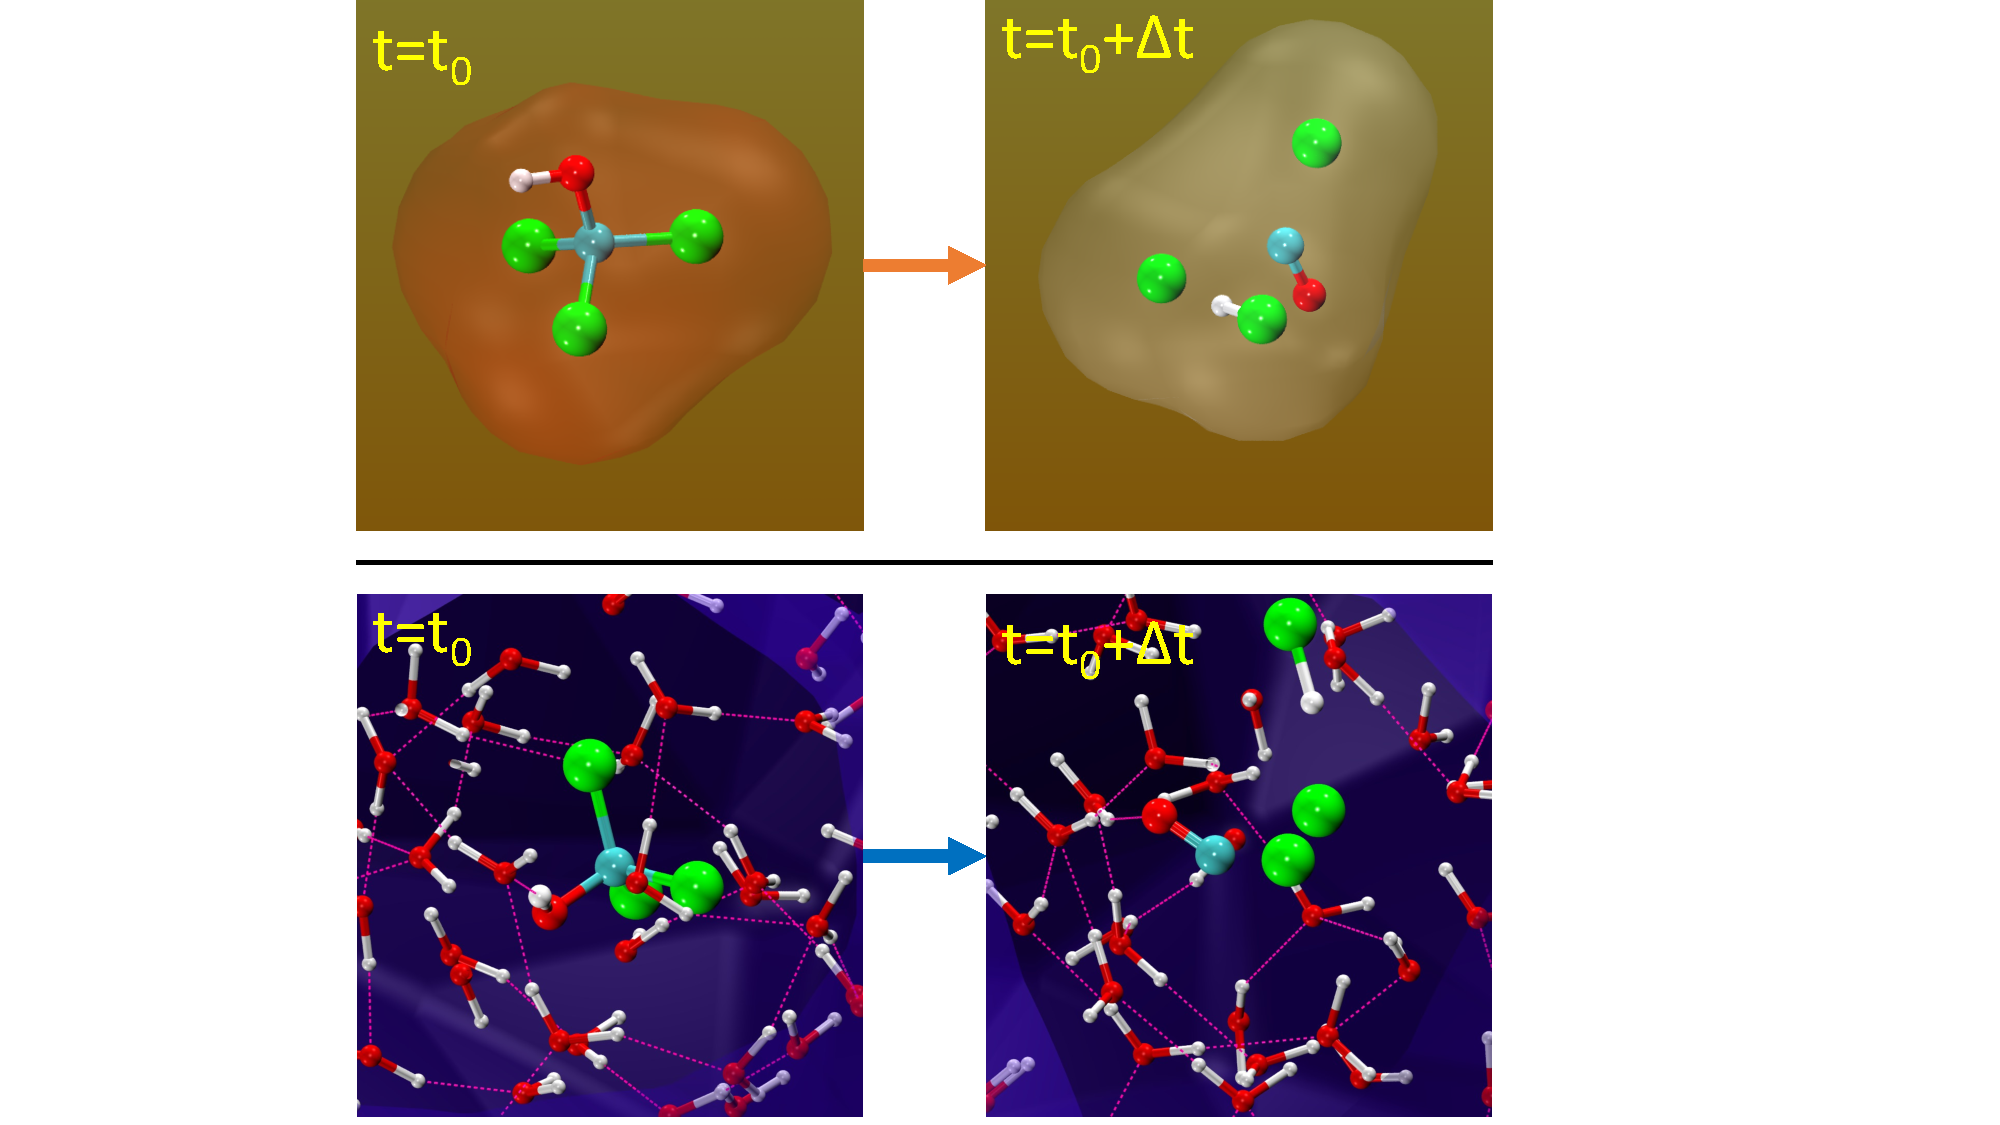
\includegraphics[width=1.0\textwidth]{images/ccl3oh-2.pdf}
   \caption{Gas-phase AIMD (top panels) and solution phase AIMD/MM (bottom panels) simulations of the decomposition of CCl$_3$OH$^{-1}$.}
   \label{fig.enviro.ccl4aimd}
\end{figure*}
Results from both these simulations clearly showed that CCl$_3$OH$^-$ immediately decomposes into carbon monoxide and chloride fragments.  AIMD and AIMD/MM simulations for the radical ion, CCl$_2$OH$^-$, also showed that it immediately decomposed as well (not shown).  Both these sets of results are in agreement with the observation that it is energetically favorable to fragment the negatively charged trichloromethanol and dichloromethanol species into a carbon monoxide and chloride species, further confirming that electron-transfer to these chloro-alcohol species may be what controls the presence of alternative pathways in the "chloroform problem".


\subsection{Reaction Pathways}
\label{subsection:app.reactionpathways}
+As illustrated in the previous section, it is quite common to hypothesize a chemical reaction network that contains multiple branching pathways that are all thermodynamically favorable.  As a result of this, relying only on reaction energies can be limiting, and approaches to modeling reaction kinetics, e.g. transition-states and reaction pathways are needed.  Unfortunately, these types of calculations involve difficult optimizations that can easily fail.  Even in best case scenarios with an expert user running the calculation, this type of calculation will still end up being 10-20 times more expensive than a reaction energy calculation.  Modeling reactions in solution is even worse.  In addition, transition-states usually contain non-bonding electronic states that are not well described by lower levels of electronic structure theories, and moreover many reactions, even intrinsic one-step reactions, end up having multiple pathways containing multiple barriers.  In short, these calculations are time-consuming and difficult, and not surprisingly, automating calculations for transition-states and reaction pathways is an active area of research.  Even though transition-state and reaction pathway calculation are not completely automated in Arrows, there are several workflows implemented in Arrows that can be used to perform these types of simulations (see the online Arrows manuals \url{https://nwchemgit.github.io/EMSL_Arrows.html#} or 
 \url{https://ebylaska.github.io/TinyArrows/}). 

\begin{figure*}[!h]
   \centering
    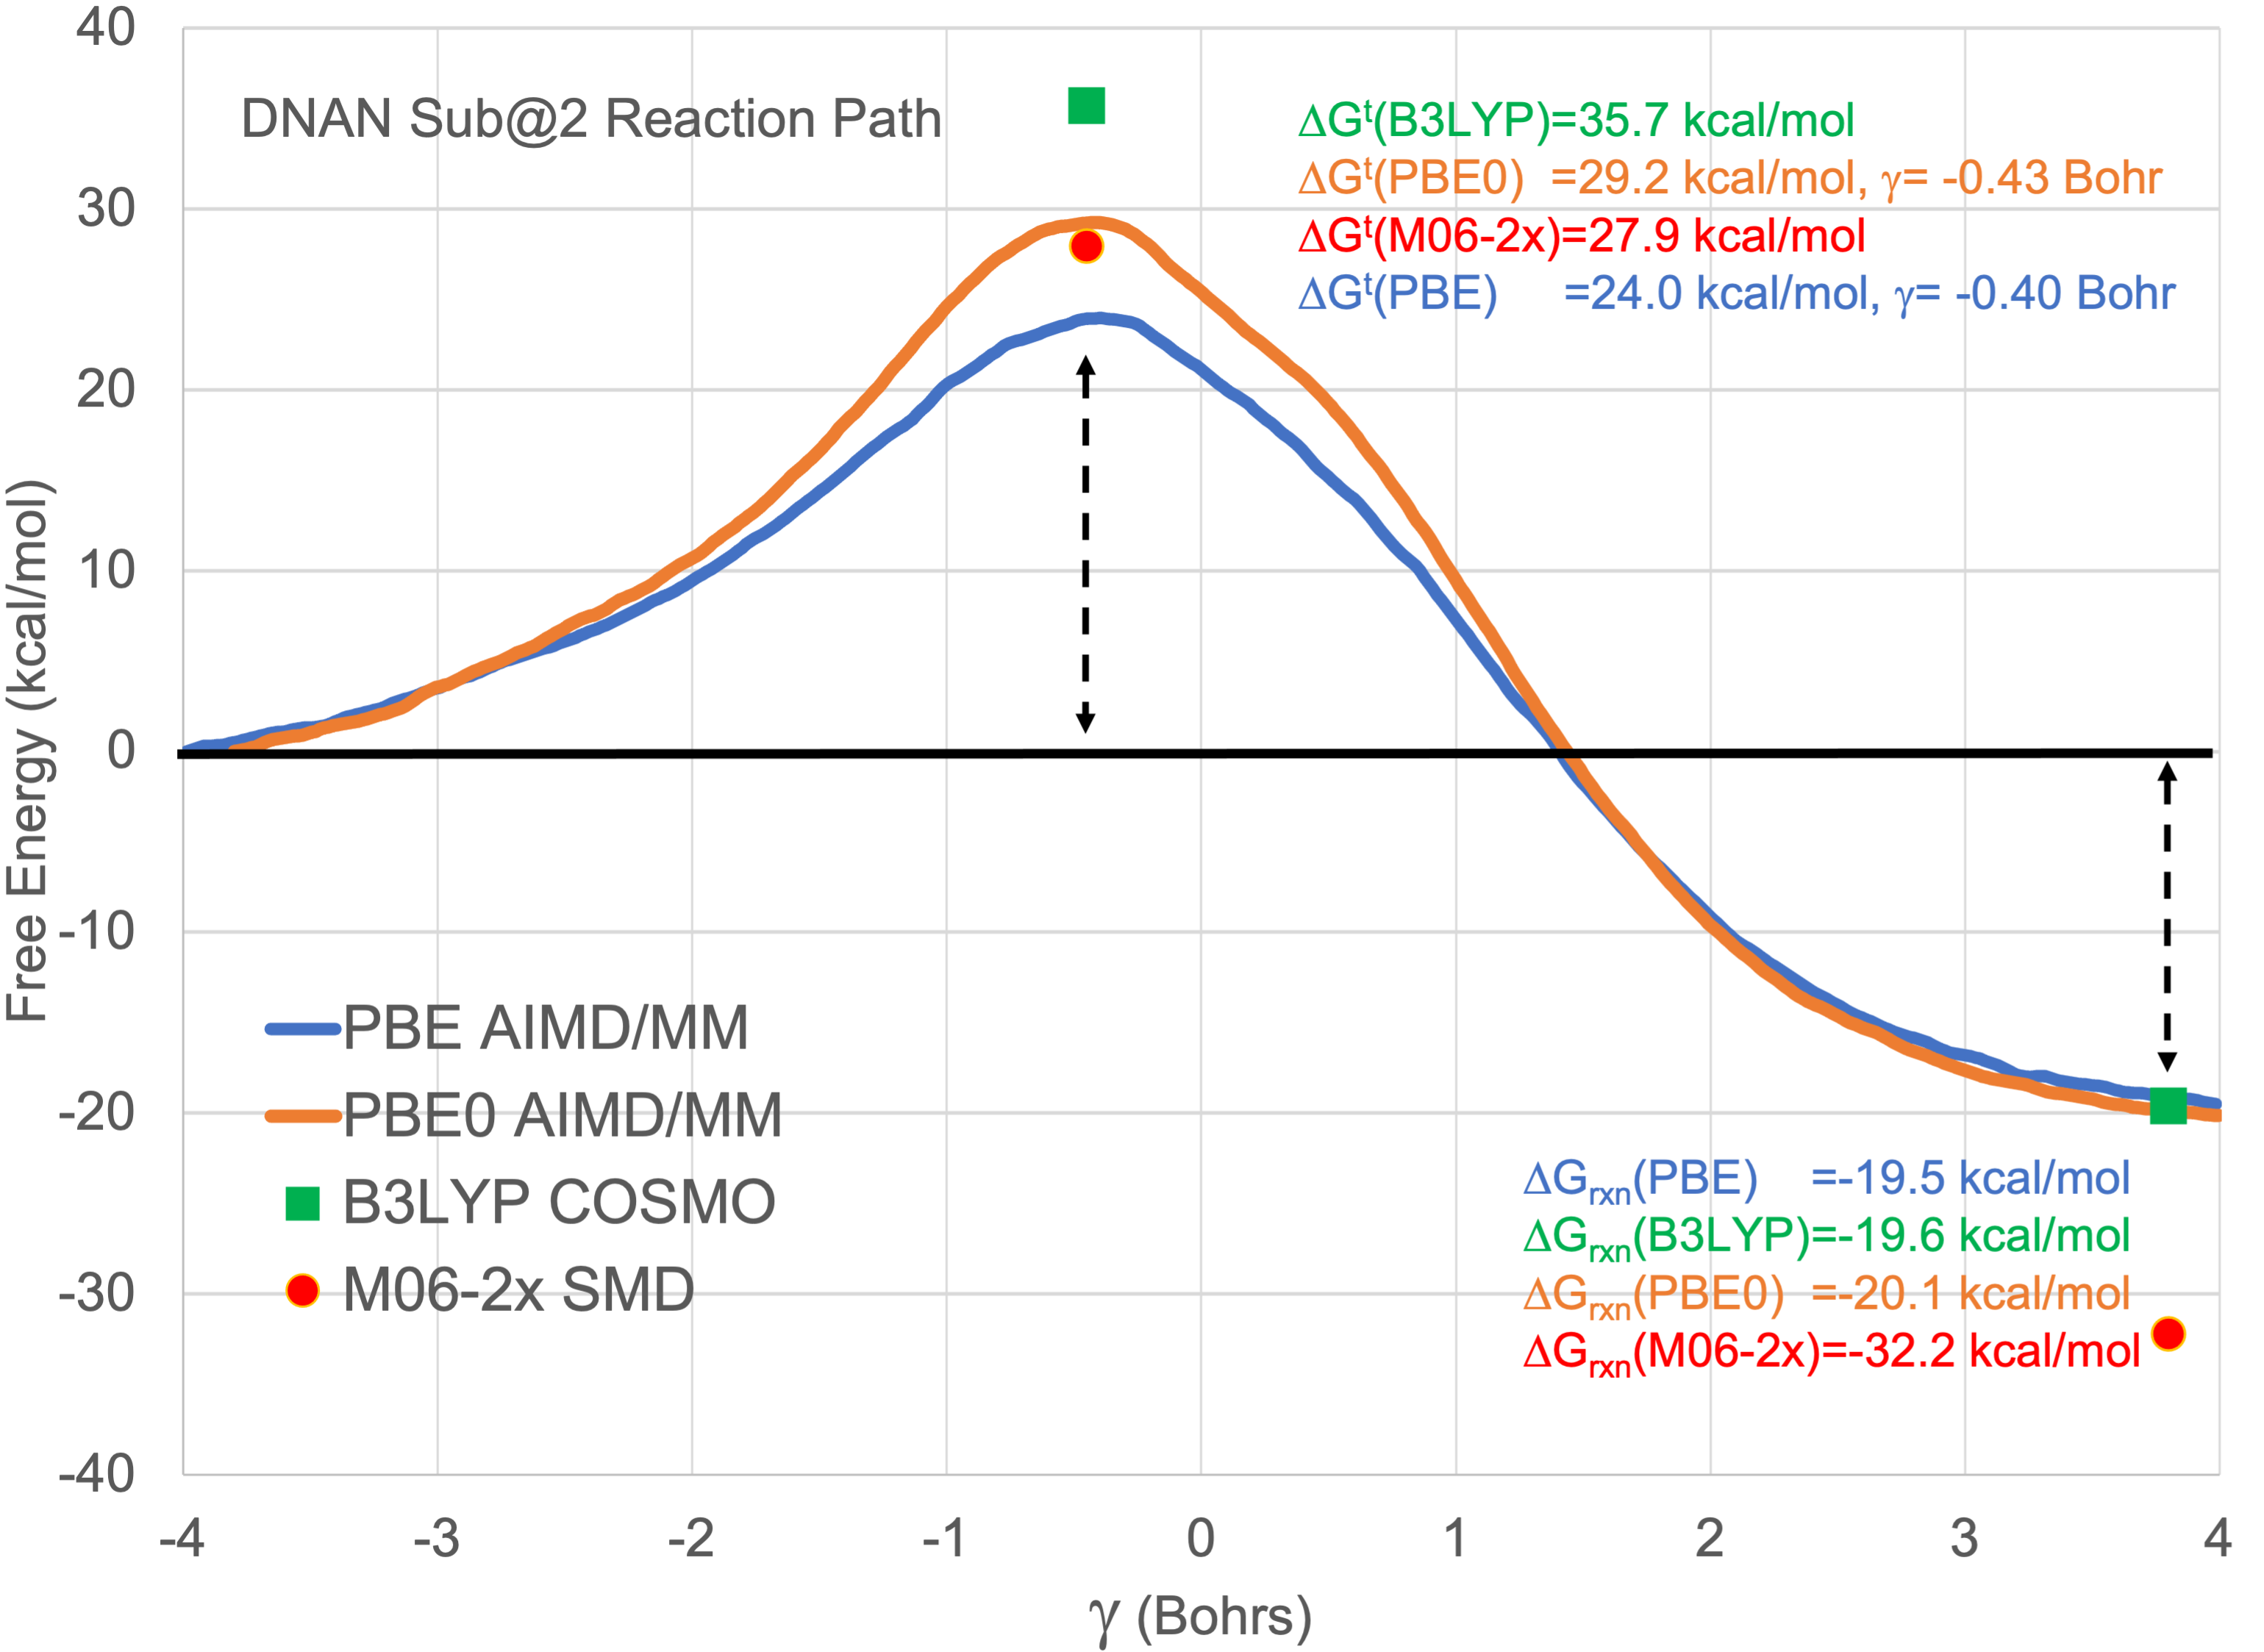
\includegraphics[width=1.0\textwidth]{images/DNAN-4-OH-pathway.png}
   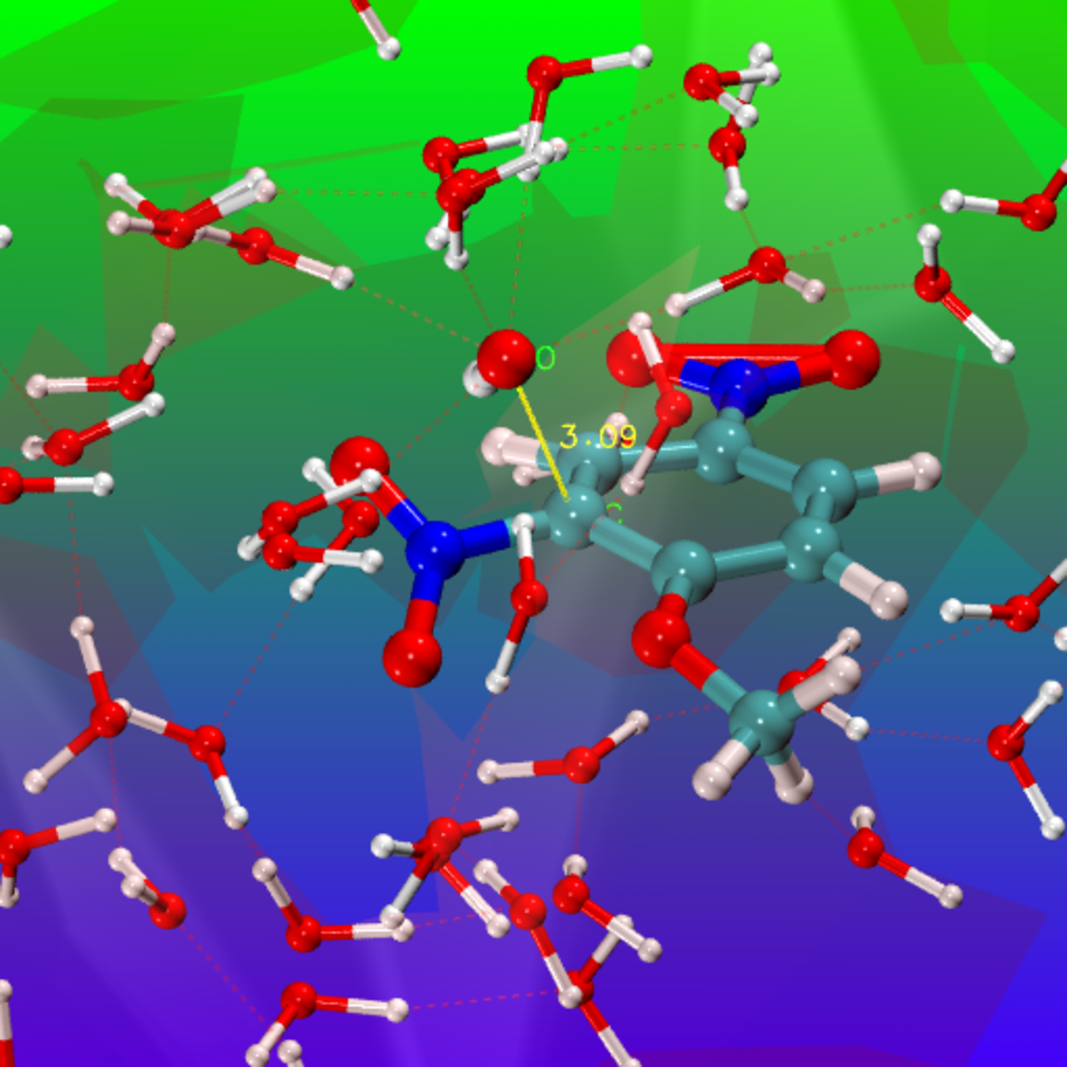
\includegraphics[width=0.32\textwidth]{images/wham30m.pdf}
   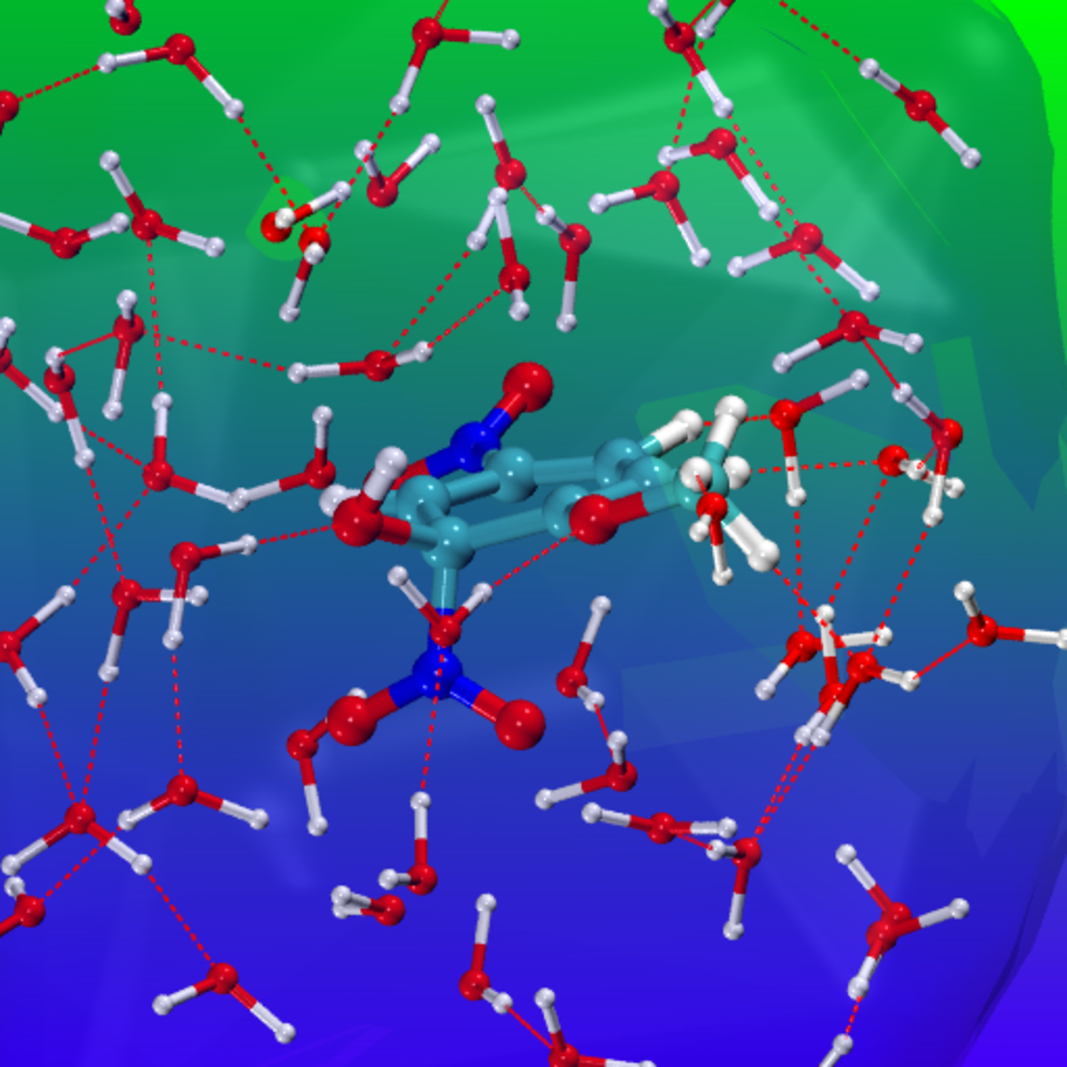
\includegraphics[width=0.32\textwidth]{images/wham00.pdf}
   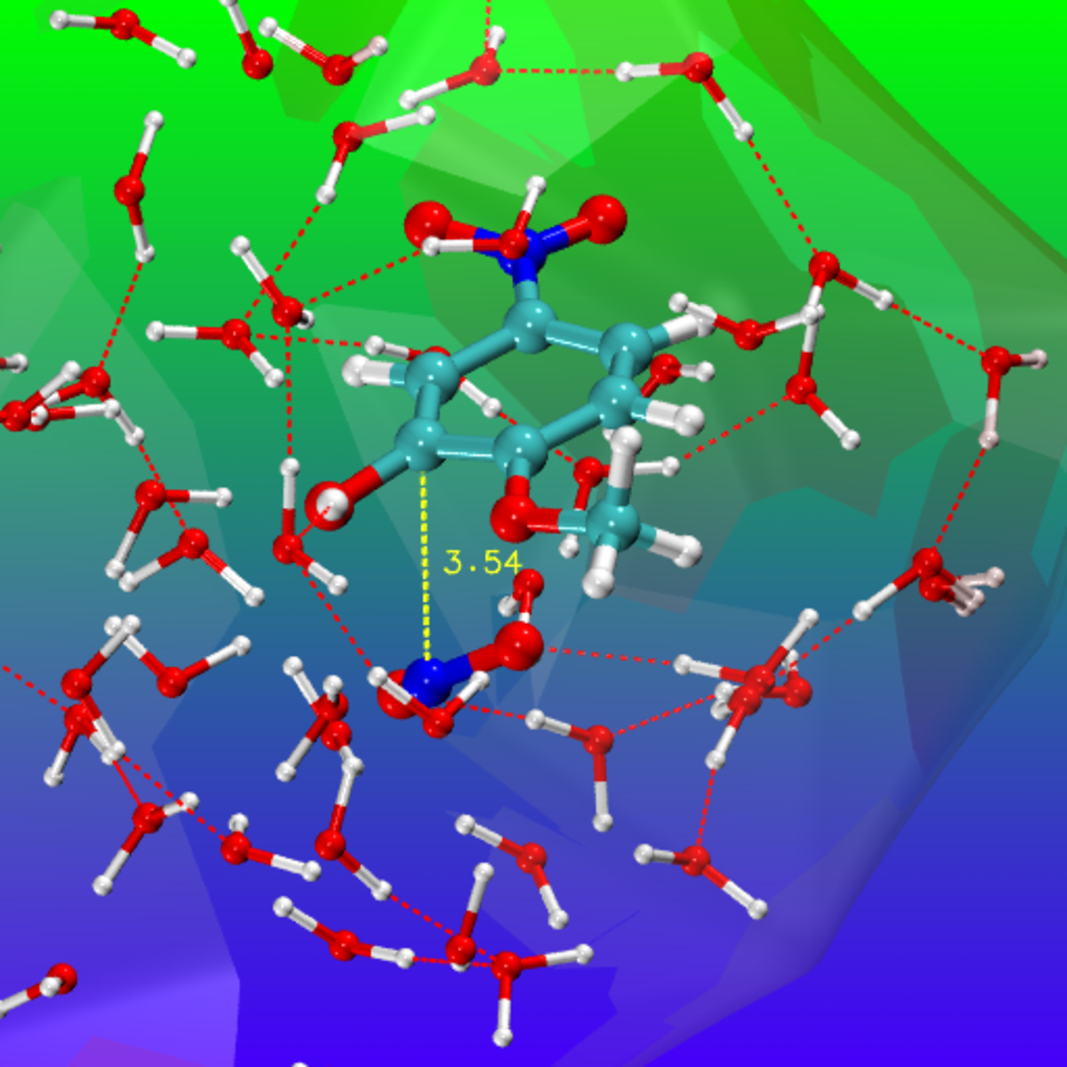
\includegraphics[width=0.32\textwidth]{images/wham40.pdf}
   \caption{(Top) Free energy reaction pathway for the 2,4-dinitroanisole + OH$^-$ $\rightarrow$ 2-methoxy-5-nitrophenol + NO$_2^-$ nucleophilic aromatic reaction of 2,4-dinitroanisole (DNAN). Also shown in the figure are results of the reaction energy and barrier from the prior calculations of Salter-Blanc et al.~\cite{salter2013mechanisms} and Hill et al.~\cite{hill2012dft}, which used the COSMO~\cite{klamt1993cosmo} and SMD~\cite{marenich2009universal} solvent models respectively to describe solvation. (Bottom) Snapshots from different windows of the WHAM simulations for the reaction.}
   \label{fig.enviro.hydrolysis}
\end{figure*}

One of the more important reactions, in which reaction pathway calculations are needed, that affects the environmental fate of most organic compounds, is alkaline hydrolysis.  Owing to its ever-presence, it is often used as a baseline against which the significance of all other environmental processes are considered. Typically, for many molecules, hydrolysis can proceed via multiple different reactions (e.g., nucleophilic aromatic substitution, hydrogen abstraction, and Meisenheimer addition reactions are important reactions for nitroaromatic hydrolysis)  that are all thermodynamically favorable, and thus it is a type of reaction for which transition-states and reaction pathways are needed.  

To illustrate using Arrows to calculate a reaction pathway for the alkaline hydrolysis of 2,4-dinitroanisole (DNAN) in solution by nucleophilic aromatic substitution are shown in Fig.~\ref{fig.enviro.hydrolysis}.
These results show that the 2,4-dinitroanisole + OH$^-$ $\rightarrow$ 2-methoxy-5-nitrophenol + NO$_2^-$ nucleophilic aromatic reaction, while strongly exothermic, has a high barrier at both the PBE~\cite{perdew1996generalized} and PBE0~\cite{adamo1999toward} levels (Note the barrier height from the PBE0 simulation is expected to be more accurate than the PBE simulation, which is usually underestimated) suggesting that it will proceed very slowly and likely be out competed by other hydrolysis reactions.  These reaction pathway simulations were performed with the weighted histogram analysis method (WHAM)~\cite{SOUAILLE200140} using the AIMD/MM~\cite{laio2002hamiltonian,cauet2010structure} method with PBE96~\cite{perdew1996generalized} and PBE0~\cite{adamo1999toward} exchange correlation functionals in a bath of 56 water molecules (i.e., 1 M concentration).  
A short write-up explaining the WHAM method and how to use it with NWChem is available for download~\cite{attafinite}.  The “bondings” collective variable, which is defined as the sum of the bond distances (in Bohr) of the bonds destroyed subtracted from the sum of bond distances (in Bohr) of the bonds created during the reaction, was used for the reaction coordinate in these calculations.

WHAM simulations are another example of a  molecular simulation that can benefit from the workflow capabilities in Arrows.  Examples of how to run WHAM and other types of free energy simulations, including potential of mean force (PMF), metadynamics, and temperature accelerated molecular dynamics (TAMD),  can be found in the online Arrows manuals (\url{https://nwchemgit.github.io/EMSL_Arrows.html#} or 
 \url{https://ebylaska.github.io/TinyArrows/}).


%\textbf{Workflow to generate an AIMD/MM WHAM Window:}
%\begin{enumerate}
%    \item Navigate to the "Arrows Periodic Builder" tab, and select the "Reaction" option. Enter a chemical reaction in the chemical reaction input, e.g., 2,4-dinitroanisole + hydroxide  \verb|-->| 2-methoxy-5-nitrophenol + nitrite.
%    \begin{itemize}
%        \item Alternatively, a chemical reaction drawn in the JSME Builder (Arrows Entry - 2D Builder (non periodic)" tab) can be placed by selecting the Use JSME Reaction button above the reaction input.
%    \end{itemize}
%
%    \item Make sure the unit cell is off by pushing the "unit cell on/off" button above the JSMol window. Then select the "Build reactants from chemical reaction" button below the reaction input to place the reactants in the JSMol builder.
%    
%    \item Select the "Generate chemical reaction hash" and "Search reaction constraints using reaction hash" buttons in sequence to generate the reaction hash and determine the reaction indexes and constraints.
%
%    \item Enter the WHAM spring constant and gamma in the WHAM\_spring and WHAM\_gamma input at the bottom of the reaction option input.
%    
%    \item To generate a window for a WHAM calculation, first select the "Generate WHAM model" button to generate an initial geometry
%   
%    \item Once step 5 is finished, select the "Generate WHAM solvated" button to the solvate the reactants.
%    
%    \item After step 6 is finished, in NWChem input deck is in the "NWChem Input Editor" tab, where it can be submitted to the Arrows nwchem\_queue, or the input deck can be downloaded.
%\end{enumerate}
%\newline


4
%There are a variety of ways to calculate the distributions.  Typically, the histogram method is used to do this type of calculations. In this work, we calculated the biased distributions with a Hausdorff moment expansion with 15 moments to improve the efficiencies of these simulations.  After the N$_w$ windows are sampled, their respective biased probability distributions are combined to yield a single unbiased probability distribution that is optimal. Once the total unbiased probability distribution is known, the free energy can be estimated.  In order for an umbrella sampling procedure to work, the number of windows along with their corresponding biasing potentials are designed to make the resulting biased probability distributions on the neighboring windows overlap. 

\section{Conclusions}
%Over the last few decades, significant progress has been made in the development and use of electronic structure and other molecular simulation methods.  As these methods become more mature and are able to simulate larger and more complex chemical simulations, the need for improvement in scientific visualization, molecular builders, simplified the input to simulation methods,  and the development of new approaches and languages to describe simulations, along with workflows to carry them out, becomes more apparent.  We have been investigating and prototyping higher-level intelligently designed web interfaces to carry out complex and difficult molecular and materials simulations.

This chapter provides a brief overview and demonstrations of the various functionalities of the Arrows web-based tools. These tools combine NWChem, SQL~\cite{chamberlin1974sequel,hursch1988sql} and NoSQL~\cite{stonebraker2010sql} databases, email, back-end web servers, external web services, and web applications, and it was designed to carry out complex and difficult molecular and materials simulations.  It was also designed to provide a starting infrastructure for researchers in molecular simulation to investigate and prototype intelligently designed web interfaces.  There are two implementations of Arrows called EMSL Arrows and TinyArrows, which are freely available. EMSL Arrows is hosted by the William R. Wiley Environmental Molecular Sciences Laboratory at PNNL, and TinyArrows is a stand-alone implementation of Arrows available on GitHub.

Currently, Arrows can be used to calculate reaction thermodynamics and reaction pathways for molecular systems, and broad range of advanced computational chemistry simulations (e.g., IR, NMR, EXAFS spectra, and free energy reaction pathways). Arrows has potential benefits to both users and developers of molecular simulation software.  For users, it makes molecular simulation more accessible, and it gives them the ability to design and carry out complex scientific workflows (e.g., AIMD-EXAFS~\cite{fulton2012near,nichols2008equatorial}, chemical reaction networks, AIMD and AIMD/MM~\cite{laio2002hamiltonian,cauet2010structure}
simulations, AIMD free energy simulations).  
Given that it is easy to run large numbers of calculations and carry out complex workflows, another potential benefit of Arrows is to help developers both improve and find bugs in their computational chemistry codes.

In the future, there are many ways that Arrows and other web-based tools could be improved.  As new molecular (exascale) simulation methods are able to handle thousands to millions of atoms, even at the level of DFT, new  ways to enter large scale chemical and materials systems will be needed.  As discussed in section~\ref{subsection:otherarrows}, reaction path generators can be made more automated, and even generalized to be reaction predictors, using algorithms and techniques from AI and ML.  Finally, several improvements could be made in modeling chemical reaction networks.  In the near future, it should become not only possible to routinely map out chemical reaction networks, but extend them with ML surrogate models that are differentiable, based on AIMD and other first principles rare event modeling. Furthermore, if AIMD rare-event modeling is coupled with multi-physics and mesoscopic models with continuum descriptions, such as classical density-functional theory, it could be possible to enable the optimization of reaction environmental conditions to obtain desired critical pathways through a chemical reaction network and vice versa (e.g., optimize catalytic processes, infer geochemical environments, develop new approaches for environmental degradation, and design new chemical processes for polymer upcycling that are able to destroy the macromolecular structures in plastics).


Finally, the goals of computational chemistry automation, as implemented by Arrows, are quickly evolving.  In our experience,  Arrows, which was initially designed to make complex calculations easier to carry out, reduce input errors, detect computational errors, aid reproducibility, provide a log of calculation workflows, and visualize results, is now allowing scientists to carry out new types of combined scientific studies, where computation and experiment are used either in tandem or in sequence to test a scientific hypothesis.







%One approach for dealing with the need for a better molecular simulation infrastructure, that has gained in popularity in recent years, is to (counterintuitively) rely even more on centralized systems of simulations and data through commercial cloud providers or web portals provided through government funded consortiums.  The fear of centralized computing and data management in molecular simulation, is that it could quickly transform from a way of making simulation better and easier to carry out through standards of data, and input and output, to putting into place rigid computational infrastructures that lead to simulation codes and algorithms disconnected from the computation hardware of the day, or even worse imagined scenarios.

%Putting into place rigid computational infrastructures that lead to simulation codes and algorithms disconnected from the computation hardware of the day, or even worse case scenarios where, not only is are simulations, as in the past, only accessible to a limited number of researchers, but a dystopian bureaucracy of simulation where there is automated judgement of a simulation's value, stagnation of new developments, and the less, rather than more, impact on science....imagined dystopian bureaucracies depicted in books and film.

\section*{Acknowledgements}
This work was supported by the NWChem project in
the DOE BER William R. Wiley Environmental Molecular Sciences Laboratory (EMSL),  the DoD Strategic Environmental Research and Development Program (SERDP) under ER1735 and ER-2725, the  U.S. Department of Energy, Office of Science, Advanced Scientific Computing Research ECP program (NWChemEx project),  and was also supported by the U.S. Department of Energy, Office of Science, Office of Basic Energy Sciences, Chemical Sciences, Geosciences, and Biosciences Division (Sandia-Livermore CCS, PNNL QIS, and PNNL Geosciences projects) DE-AC05-76RL01830.  EMSL operations are supported by the DOE's Office of Biological and Environmental Research. This research used resources of the National Energy Research Scientific Computing Center (NERSC), a User Facility supported by the Office of Science of the U.S. DOE under Contract No. DE-AC02-05CH11231, to carry out the AIMD-EXAFS studies highlighted in this work.
This report has not been subject to review by SERDP and therefore does not necessarily reflect their views and no official endorsement should be inferred.


\section*{Author Contributions}
E.J.B. was the primary author of the manuscript, and he developed the EMSL Arrows and Tiny Arrows software.  D.S. and T.L.S helped test and debug the Arrows software. All authors have read and contributed to the editing of the manuscript, and all authors have provided feedback to the design and implementation of Arrows.  E.J.B. and  D.S. carried out the AIMD-EXAFS simulations and E.S.I analyzed the AIMD-EXAFS results given in section~\ref{sec:geochemistry}. T.L.S. and P.G.T. generated Fig.~\ref{fig.intro.rxnnetwork}. 
S.O. with E.J.B. led the deployment of EMSL Arrows at Pacific Northwest National Laboratory.  S.O. was also responsible for installing and testing the HTTP security protocols used for accessing the  EMSL Arrows Web APIs.

\section*{Conflict of Interest}
The authors declare that they have no competing interests.



%%%%%%%%%%%%%%%%%%%%%%%%%%%%%%%%%%%%%%%%%%%%%%%%%%%%%%%%%%%%%%%%%%%%%%%%%%%%%%%%%%%%%%%%%%%%%%%%%%%%%%%%%%%%%
%%%%%%%%%%%%%%%%%%%%%%%%%%%%%%%%%%%%%%%%%%%%%%%%%%%%%%%%%%%%%%%%%%%%%%%%%%%%%%%%%%%%%%%%%%%%%%%%%%%%%%%%%%%%%

\clearpage


%%%%%%%%%%%%%%%%%%%%%%%%%%%%%%%%%%%%%%%%%%%%%%%%%%%%%%%%%%%%%%%%%%%%%%%%%%%%%%%%%%%%%%%%%%%%%%%%%%%%%%%%%%%%%
%%%%%%%%%%%%%%%%%%%%%%%%%%%%%%%%%%%%%%%%%%%%%%%%%%%%%%%%%%%%%%%%%%%%%%%%%%%%%%%%%%%%%%%%%%%%%%%%%%%%%%%%%%%%%
%\bibliographystyle{plain}
\bibliographystyle{unsrt}
\bibliography{EMSL-Arrows}



%\section*{Acronyms}
%
%\begin{acronym}
%  \acro{AIMD}{Ab initio molecular dynamics}
%  \acro{AIMD/MM}{Hybrid ab initio molecular dynamics molecular dynamics} 
%  \acro{API}{}
%  \acro{CCl$_4$}{}
%  \acro{CCSD(T)}{Coupled cluster singles and double with perturbative triples} 
%  \acro{DFT}{Density functional theory}
%  \acro{EMSL}{}
%  \acro{EXAFS}{}
%  \acro{HTML5}{}
%  \acro{HTTP}{}
%  \acro{IR}{}
%  \acro{JSMol}{}
%  \acro{NWChem}{North West Chemistry program}
%  \acro{Mopac}{}
%  \acro{NMR}{}
%  \acro{NoSQL}{}
%  \acro{Plane-Wave DFT}{Plane-wave density functional theory method}
%  \acro{PAW}{Projector augmented plane-wave method}
%  \acro{PBE0}{}
%  \acro{PBE96}{}
%  \acro{PSPW}{pseudopotential plane-wave density functional theory method} 
%  \acro{SQL}{}
%  \acro{TCP}{}
%  \acro{web app}{}
%  \acro{EPA-CTS}{}
%  \acro{EAWAG-BBD}{}
%  \acro{KinBot}{}
%  \acro{RMG}{}
%  \acro{IBM RXN}{}
%  \acro{PNNL}{}
%  \acro{TinyArrows}{} 
%  \acro{GitHub}{}
%  \acro{QIS}{}
%  \acro{XYZ}{}
%  \acro{JSON}{}
%  \acro{SMILES}{}
%  \acro{IUPAC}{}
%  \acro{KEGG}{}
%  \acro{CAS}{}
%  \acro{PubChem}{}
%  \acro{ChemSpider}{}
%  \acro{ChEMBL}{}
%  \acro{InChI}{} 
%\end{acronym}

\end{document}
